\documentclass[preprint]{elsarticle}

\usepackage{hyperref}

\usepackage[english]{babel}
\usepackage[utf8]{inputenc}
\usepackage[T1]{fontenc}

\usepackage{amsmath}  % Maths
\usepackage{amsfonts} % Maths
\usepackage{amssymb}  % Maths
\usepackage{stmaryrd} % Maths (crochets doubles)

\usepackage{url}     % Mise en forme + liens pour URLs
\usepackage{array}   % Tableaux évolués

\usepackage{comment}


\usepackage{prettyref}
\newrefformat{def}{Def.~\ref{#1}}
\newrefformat{fig}{Fig.~\ref{#1}}
\newrefformat{pro}{Property~\ref{#1}}
\newrefformat{pps}{Proposition~\ref{#1}}
\newrefformat{lem}{Lemma~\ref{#1}}
\newrefformat{thm}{Theorem~\ref{#1}}
\newrefformat{sec}{Sect.~\ref{#1}}
\newrefformat{ssec}{Subsect.~\ref{#1}}
\newrefformat{sssec}{Subsect.~\ref{#1}}
\newrefformat{suppl}{Appendix~\ref{#1}}
\newrefformat{eq}{Eq.~\eqref{#1}}
\newrefformat{ex}{Example~\ref{#1}}
\newrefformat{tb}{Table~\ref{#1}}
\def\pref{\prettyref}

\newdefinition{definition}{Definition}
\newdefinition{property}{Property}
\newdefinition{proposition}{Proposition}
\newdefinition{example}{Example}

\usepackage{tikz}
\newdimen\pgfex
\newdimen\pgfem
\usetikzlibrary{arrows,shapes,shadows,scopes}
\usetikzlibrary{positioning}
\usetikzlibrary{matrix}
\usetikzlibrary{decorations.text}
\usetikzlibrary{decorations.pathmorphing}

% Macros relatives à la traduction de PH avec arcs neutralisants vers PH à k-priorités fixes

% Macros générales
\def\Pint{\textsc{PINT}}

% Notations générales pour PH
\newcommand{\PH}{\mathcal{PH}}
\newcommand{\PHs}{\Sigma}
\newcommand{\PHl}{L}
%\newcommand{\PHp}{\mathcal{P}}
\newcommand{\PHp}{\textcolor{red}{\mathcal{P}}}
\newcommand{\PHproc}{\mathcal{P}}
\newcommand{\PHa}{\PHh}
\newcommand{\PHh}{\mathcal{H}}
\newcommand{\PHn}{\mathcal{N}}

\newcommand{\PHhitter}{\mathsf{hitter}}
\newcommand{\PHtarget}{\mathsf{target}}
\newcommand{\PHbounce}{\mathsf{bounce}}
\newcommand{\PHsort}{\Sigma}

\def\f#1{\mathsf{#1}}
\def\focals{\f{focals}}
\def\play{\cdot}
\def\configs#1{\mathbb C_{#1\rightarrow a}}

%\newcommand{\PHfrappeR}{\textcolor{red}{\rightarrow}}
%\newcommand{\PHmonte}{\textcolor{red}{\Rsh}}

\newcommand{\PHfrappeA}{\rightarrow}
\newcommand{\PHfrappeB}{\Rsh}
%\newcommand{\PHfrappe}[3]{\mbox{$#1\PHfrappeA#2\PHfrappeB#3$}}
%\newcommand{\PHfrappebond}[2]{\mbox{$#1\PHfrappeB#2$}}
\newcommand{\PHfrappe}[3]{#1\PHfrappeA#2\PHfrappeB#3}
\newcommand{\PHfrappebond}[2]{#1\PHfrappeB#2}
\newcommand{\PHobjectif}[2]{\mbox{$#1\PHfrappeB^*\!#2$}}
\newcommand{\PHconcat}{::}
\newcommand{\PHneutralise}{\rtimes}

\def\PHget#1#2{{#1[#2]}}
%\newcommand{\PHchange}[2]{#1\langle #2 \rangle}
\newcommand{\PHchange}[2]{(#1 \Lleftarrow #2)}
\newcommand{\PHarcn}[2]{\mbox{$#1\PHneutralise#2$}}
\newcommand{\PHjoue}{\cdot}

\newcommand{\PHetat}[1]{\mbox{$\langle #1 \rangle$}}


% Notations spécifiques à ce papier
\newcommand{\PHdirectpredec}[1]{\PHs^{-1}(#1)}
\newcommand{\PHpredec}[1]{\f{pred}(#1)}
\newcommand{\PHpredecgene}[1]{\f{reg}({#1})}
\newcommand{\reg}{\PHpredecgene}
\newcommand{\PHpredeccs}[1]{\PHpredec{#1} \setminus \Gamma}

\newcommand{\PHincl}[2]{#1 :: #2}

\def\ctx{\varsigma}
\def\ctxOverride{\Cap}
\def\state#1{\langle #1 \rangle}

% Notations spécifiques aux graphes d'états
%\newcommand{\PHge}{\textcolor{red}{\mathcal{GE}}}
%\newcommand{\PHt}{\mathcal{T}}
%\newcommand{\GE}{\mathcal{GE}}
%\newcommand{\GEt}{\mathcal{T}}
%\newcommand{\GEl}{\PHl}
%\newcommand{\GEa}{\PHa}
%\newcommand{\GEva}[3]{#1 \stackrel{#2}{\longrightarrow} #3}
%\newcommand{\GEval}[3]{#1 \stackrel{#2}{\Longrightarrow} #3}
%\newcommand{\GEget}[2]{\PHget{#1}{#2}}


\def\DEF{\stackrel{\Delta}=}
\def\EQDEF{\stackrel{\Delta}\Leftrightarrow}
\def\SUBSETDEF{\stackrel{\Delta}\subset}

\newcommand{\segmllabel}{\llbracket}
\newcommand{\segmrlabel}{\rrbracket}
\newcommand{\segm}[2]{\segmllabel #1 ; #2 \segmrlabel}
\newcommand{\leqsegm}{\leq_{\segmllabel\segmrlabel}}
\newcommand{\ltsegm}{<_{\llbracket\rrbracket}}

\newcommand{\irB}{B}
\newcommand{\irF}{F}

\usepackage{ifthen}
\usepackage{tikz}
\usetikzlibrary{arrows,shapes}

\definecolor{lightgray}{rgb}{0.8,0.8,0.8}
\definecolor{lightgrey}{rgb}{0.8,0.8,0.8}

\tikzstyle{boxed ph}=[]
\tikzstyle{sort}=[fill=lightgray,rounded corners]
\tikzstyle{process}=[circle,draw,minimum size=15pt,fill=white,
font=\footnotesize,inner sep=1pt]
\tikzstyle{black process}=[process, fill=black,text=white, font=\bfseries]
\tikzstyle{gray process}=[process, draw=black, fill=lightgray]
\tikzstyle{current process}=[process, draw=black, fill=lightgray]
\tikzstyle{process box}=[white,draw=black,rounded corners]
\tikzstyle{tick label}=[font=\footnotesize]
\tikzstyle{tick}=[black,-]%,densely dotted]
\tikzstyle{hit}=[->,>=angle 45]
\tikzstyle{selfhit}=[min distance=30pt,curve to]
\tikzstyle{bounce}=[densely dotted,->,>=latex]
\tikzstyle{hl}=[font=\bfseries,very thick]
\tikzstyle{hl2}=[hl]
\tikzstyle{nohl}=[font=\normalfont,thin]

\newcommand{\currentScope}{}
\newcommand{\currentSort}{}
\newcommand{\currentSortLabel}{}
\newcommand{\currentAlign}{}
\newcommand{\currentSize}{}

\newcounter{la}
\newcommand{\TSetSortLabel}[2]{
  \expandafter\repcommand\expandafter{\csname TUserSort@#1\endcsname}{#2}
}
\newcommand{\TSort}[4]{
  \renewcommand{\currentScope}{#1}
  \renewcommand{\currentSort}{#2}
  \renewcommand{\currentSize}{#3}
  \renewcommand{\currentAlign}{#4}
  \ifcsname TUserSort@\currentSort\endcsname
    \renewcommand{\currentSortLabel}{\csname TUserSort@\currentSort\endcsname}
  \else
    \renewcommand{\currentSortLabel}{\currentSort}
  \fi
  \begin{scope}[shift={\currentScope}]
  \ifthenelse{\equal{\currentAlign}{l}}{
    \filldraw[process box] (-0.5,-0.5) rectangle (0.5,\currentSize-0.5);
    \node[sort] at (-0.2,\currentSize-0.4) {\currentSortLabel};
   }{\ifthenelse{\equal{\currentAlign}{r}}{
     \filldraw[process box] (-0.5,-0.5) rectangle (0.5,\currentSize-0.5);
     \node[sort] at (0.2,\currentSize-0.4) {\currentSortLabel};
   }{
    \filldraw[process box] (-0.5,-0.5) rectangle (\currentSize-0.5,0.5);
    \ifthenelse{\equal{\currentAlign}{t}}{
      \node[sort,anchor=east] at (-0.3,0.2) {\currentSortLabel};
    }{
      \node[sort] at (-0.6,-0.2) {\currentSortLabel};
    }
   }}
  \setcounter{la}{\currentSize}
  \addtocounter{la}{-1}
  \foreach \i in {0,...,\value{la}} {
    \TProc{\i}
  }
  \end{scope}
}

\newcommand{\TTickProc}[2]{ % pos, label
  \ifthenelse{\equal{\currentAlign}{l}}{
    \draw[tick] (-0.6,#1) -- (-0.4,#1);
    \node[tick label, anchor=east] at (-0.55,#1) {#2};
   }{\ifthenelse{\equal{\currentAlign}{r}}{
    \draw[tick] (0.6,#1) -- (0.4,#1);
    \node[tick label, anchor=west] at (0.55,#1) {#2};
   }{
    \ifthenelse{\equal{\currentAlign}{t}}{
      \draw[tick] (#1,0.6) -- (#1,0.4);
      \node[tick label, anchor=south] at (#1,0.55) {#2};
    }{
      \draw[tick] (#1,-0.6) -- (#1,-0.4);
      \node[tick label, anchor=north] at (#1,-0.55) {#2};
    }
   }}
}
\newcommand{\TSetTick}[3]{
  \expandafter\repcommand\expandafter{\csname TUserTick@#1_#2\endcsname}{#3}
}

\newcommand{\myProc}[3]{
  \ifcsname TUserTick@\currentSort_#1\endcsname
    \TTickProc{#1}{\csname TUserTick@\currentSort_#1\endcsname}
  \else
    \TTickProc{#1}{#1}
  \fi
  \ifthenelse{\equal{\currentAlign}{l}\or\equal{\currentAlign}{r}}{
    \node[#2] (\currentSort_#1) at (0,#1) {#3};
  }{
    \node[#2] (\currentSort_#1) at (#1,0) {#3};
  }
}
\newcommand{\TSetProcStyle}[2]{
  \expandafter\repcommand\expandafter{\csname TUserProcStyle@#1\endcsname}{#2}
}
\newcommand{\TProc}[1]{
  \ifcsname TUserProcStyle@\currentSort_#1\endcsname
    \myProc{#1}{\csname TUserProcStyle@\currentSort_#1\endcsname}{}
  \else
    \myProc{#1}{process}{}
  \fi
}

\newcommand{\repcommand}[2]{
  \providecommand{#1}{#2}
  \renewcommand{#1}{#2}
}
\newcommand{\THit}[5]{
  \path[hit] (#1) edge[#2] (#3#4);
  \expandafter\repcommand\expandafter{\csname TBounce@#3@#5\endcsname}{#4}
}
\newcommand{\TBounce}[4]{
  (#1\csname TBounce@#1@#3\endcsname) edge[#2] (#3#4)
}

\newcommand{\TState}[1]{
  \foreach \proc in {#1} {
    \node[current process] (\proc) at (\proc.center) {};
  }
}

% Macros spécifiques au Modèle de Thomas / aux RRB

% Notations pour le modèle de Thomas (depuis thèse)
\newcommand{\GRN}{\mathcal{GRN}}
\newcommand{\IG}{\mathcal{G}}
%\def\IG{\mathrm{IG}}
\newcommand{\GRNreg}[1]{\Gamma^{-1}(#1)}
\newcommand{\GRNres}[2]{\mathsf{Res}_{#1}(#2)}
\newcommand{\GRNallres}[1]{\mathsf{Res}_{#1}}
\newcommand{\GRNget}[2]{\PHget{#1}{#2}}
\newcommand{\GRNetat}[1]{\PHetat{#1}}

\def\levels{\mathsf{levels}}
\def\levelsA#1#2{\levels_+(#1\rightarrow #2)}
\def\levelsI#1#2{\levels_-(#1\rightarrow #2)}
%\newcommand{\PHres}{\mathsf{Res}}

\newcommand{\Kinconnu}{\emptyset}
\newcommand{\RRGva}[3]{#1 \stackrel{#2}{\longrightarrow} #3}
\newcommand{\RRGgi}{\mathcal{G}}
\newcommand{\RRGreg}[1]{\RRGgi_{#1}}



%\definecolor{darkred}{rgb}{0.5,0,0}
%\definecolor{lightred}{rgb}{1,0.8,0.8}
%\definecolor{lightgreen}{rgb}{0.7,1,0.7}
\definecolor{darkgreen}{rgb}{0,0.5,0}
%\definecolor{darkyellow}{rgb}{0.5,0.5,0}
%\definecolor{lightyellow}{rgb}{1,1,0.6}
%\definecolor{darkcyan}{rgb}{0,0.6,0.6}
%\definecolor{darkorange}{rgb}{0.8,0.2,0}

%\definecolor{notsodarkgreen}{rgb}{0,0.7,0}

%\definecolor{coloract}{rgb}{0,1,0}
%\definecolor{colorinh}{rgb}{1,0,0}
\colorlet{coloract}{darkgreen}
\colorlet{colorinh}{red}
%\colorlet{coloractgray}{lightgreen}
%\colorlet{colorinhgray}{lightred}
%\colorlet{colorinf}{darkgray}
%\colorlet{coloractgray}{lightgreen}
%\colorlet{colorinhgray}{lightred}

%\colorlet{colorgray}{lightgray}


\tikzstyle{grn}=[every node/.style={circle,draw=black,outer sep=2pt,minimum
                size=15pt,text=black}, node distance=1.5cm]
\tikzstyle{act}=[->,draw=black,thick,color=black]
\tikzstyle{inh}=[>=|,-|,draw=black,thick, text=black,label]
%\tikzstyle{inh}=[>=|,-|,draw=colorinh,thick, text=black,label]
%\tikzstyle{act}=[->,>=triangle 60,draw=coloract,thick,color=coloract]
%\tikzstyle{inhgray}=[>=|,-|,draw=colorinhgray,thick, text=black,label]
%\tikzstyle{actgray}=[->,>=triangle 60,draw=coloractgray,thick,color=coloractgray]
\tikzstyle{inf}=[->,draw=colorinf,thick,color=colorinf]
%\tikzstyle{elabel}=[fill=none, above=-1pt, sloped,text=black, minimum size=10pt, outer sep=0, font=\scriptsize,draw=none]
\tikzstyle{elabel}=[fill=none,text=black, above=-2pt,%sloped,
minimum size=10pt, outer sep=0, font=\scriptsize, draw=none]
%\tikzstyle{elabel}=[]
\tikzstyle{sg}=[every node/.style={outer sep=2pt,minimum
                size=15pt,text=black}, node distance=2cm]



% Commandes À FAIRE
%\usepackage{color} % Couleurs du texte
%\newcommand{\warnul}[1]{\textcolor{red}{\underline{#1}}}
%\newcommand{\rewriteng}[1]{\textcolor{blue}{#1}}
%\newcommand{\rewriteil}[1]{\rewriteng{\textbf{[#1]}}}
%\newcommand{\rewrite}[1]{\rewriteil{REWRITE: #1}}
%\newcommand{\towrite}[1]{\rewriteil{TOWRITE: #1}}
\newcommand{\todo}[1]{\textcolor{red}{\textbf{[TODO: #1]}}}
%\newcommand{\new}[1]{\textcolor{darkgreen}{\textbf{[$^\bigstar$New:} #1\textbf{$^\bigstar$]}}}
\def\updated#1{{\color{magenta}#1}}
\newcommand{\updatedmax}[1]{{\color{violet}#1}}
%\newcommand{\new}[1]{#1}



% Id est
\newcommand{\ie}{i.e.~}

% Césures
\hyphenation{pa-ra-me-tri-za-tion}
\hyphenation{pa-ra-me-tri-za-tions}



\begin{document}

\begin{frontmatter}

\title{Constructing Biological Regulatory Networks from Process Hitting models}
%\\\rewriteil{Or possibly: “Complementarity between PH, IG and Thomas modeling”}

\author[irccyn,nii]{Maxime Folschette}
\ead{Maxime.Folschette@irccyn.ec-nantes.fr}
\author[eth]{Lo\"ic Paulev\'e}
\author[nii]{Katsumi Inoue}
\author[irccyn,nii]{Morgan Magnin}
\author[irccyn]{Olivier Roux}

\address[irccyn]{LUNAM Universit\'e, \'Ecole Centrale de Nantes, IRCCyN UMR CNRS 6597\\
(Institut de Recherche en Communications et Cybern\'etique de Nantes)\\
1 rue de la No\"e - B.P. 92101 - 44321 Nantes Cedex 3, France.}
\address[nii]{National Institute of Informatics,\\
2-1-2, Hitotsubashi, Chiyoda-ku, Tokyo 101-8430, Japan.}
\address[eth]{BISON group, Automatic Control Laboratory, ETH Zürich\\
Physikstrasse 3, 8092 Zurich, Switzerland.}

\begin{abstract}
\parindent 0.5cm
The Process Hitting (PH) is a recently introduced framework to model concurrent processes.
Its major originality lies in a specific restriction on the causality of actions, which
makes the formal analysis of very large systems tractable.
PH is suitable to model Biological Regulatory Networks (BRNs) with complete or partial
knowledge of cooperations between regulators by defining the most permissive dynamics
with respect to these constraints.

On the other hand, the qualitative modeling of BRNs has been widely addressed using Ren\'e Thomas'
formalism, leading to numerous theoretical work and practical tools to understand emerging behaviors.

This paper establishes formal links between these two formalisms, permitting to appreciate their
complementary features.
First, the inference of the Interaction Graph (IG) from a PH models allows a compact representation of
the regulations that are effective for the dynamics.
From this IG, well-known results can be applied to derive global dynamical properties for the
modelled BRN.
Second, the inference of all Thomas models that are compatible with a given PH is tackled.
As the PH allows partial specification of cooperation between components, this inference
emphasizes the ability of PH to deal with large BRNs with incomplete knowledge on
cooperations, where Thomas' approach fails because of the combinatorics of parameters.

The inference of corresponding Thomas' models is provided using Answer Set Programming,
which allows notably an efficient enumeration of (possibly numerous) compatible parametrizations.
\todo{application}
\end{abstract}

\end{frontmatter}



\section{Introduction}\label{sec:intro}
As regulatory phenomena play a crucial role in biological systems, they need to be studied accurately.
Biological Regulatory Networks (BRNs) consist in sets of either positive or negative mutual effects between the components.
With the purpose of analyzing these systems, they are often modeled as graphs which make it possible to determine the possible evolutions of all the interacting components of the system.
Indeed, besides continuous models of physicists, often designed through systems of ordinary
differential equations, a discrete modeling approach was initiated by René Thomas in 1973
\cite{Thomas73}.

In this approach, the different levels of a component, such as concentration or expression levels, are abstractly represented by (positive) integer values and transitions between these levels may be considered as instantaneous.
Hence, qualitative state graphs may be derived from which we are able to formally find out all the possible behaviors expressed as sequences of transitions between these states.
Nevertheless, these dynamics can be precisely established only with regard to some discrete parameters,
hereafter called ``Thomas' parameters'',
which stand for kinds of ``focal points'', i.e. the evolutionary tendency from each state and depending on the set of the other currently interacting components.
%resources in this very state, that is, the set of the other currently interacting components.
%Hereafter, we refer to these discrete parameters as Thomas' parameters.

Thomas' modeling has motivated numerous works around the link between the Interaction Graph (IG)
(summarizing the global influences between components) and the possible dynamics (e.g.,
\cite{RiCo07,RRT08}),
model reduction (e.g., \cite{Naldi09}), formal checking of dynamics (e.g., \cite{Richard06,Naldi07}), 
and the incorporation of time (e.g., \cite{Siebert06,Ahmad08}) and probability
(e.g., \cite{Twardziok10-CMSB}) dimensions, to name but a few.
While the formal checking of dynamical properties is often limited to small networks because of the
state graph explosion, the main drawback of this framework is the difficulty to specify Thomas'
parameters, especially for large networks.

In order to address the formal checking of dynamical properties within very large BRNs, we recently
introduced in \cite{PMR10-TCSB} a new formalism, named the \emph{``Process Hitting''} (PH), to model
concurrent systems having components with a few qualitative levels.
A PH describes, in an atomic manner, the possible evolutions of a process (representing one
component at one level) triggered by the hit of at most one other process in the system.
This framework can be seen as a special class of formalisms like Petri Nets or Communicating Finite
State Machines, where the causality between actions is restricted.
Thanks to the particular structure of interactions within a PH, very efficient static analysis
methods have been developed to over- and under-approximate reachability properties making tractable
the formal analysis of BRNs with hundreds of components \cite{PMR12-MSCS}.

PH is suitable to model BRNs with different levels of abstraction in the specification of
cooperations (associated influences) between components.
This allows to model BRNs with a partial knowledge on precise evolution functions for components
by capturing the largest (the most general) dynamics.

The objectives of the work presented in this paper are the following.
Firstly, we show that starting from one PH model, it is possible to find back the underlying IG.
We perform an exhaustive search for the possible interactions on one component from all the
others, consistently with the knowledge of the dynamics that these interactions lead to and that are
expressed in PH.
The second phase of our work concerns the Thomas' parameters inference.
It consists in determining the nesting set (possibly too large) of the parameters which necessarily
lead to the satisfaction of the known cooperating constraints.
The resulting BRN dynamics is ensured to respect the PH dynamics, \ie no spurious transitions are
made possible by the inference.
Answer Set Programming (ASP) \cite{Baral03} turns out to be effective for these enumerative searches.

The outcome of this work is twofold.
The first benefit is that such an approach makes it possible to refine the construction of
BRNs with a partial and progressively brought knowledge in PH, while being able to export such
models in the Thomas' framework.
This work thus strengthens the formal link between both modelings.
The second feature of our method is that it can be applied on very large BRNs.

Finally, it must be noticed that we are not interested in this paper in the derivation of one
PH from a BRN (which was previously described in \cite{PMR10-TCSB}) but, on the contrary, to finding out
a set of BRNs from one PH.

Our work is related to the approach of \cite{Khalis09} which relies on temporal logic, and \cite{20646302,DBLP:conf/ipcat/CorblinFTCT12} which also uses constraint programming. Both aim at determining a class of models which are consistent with available partial data on the regulatory structure and dynamical properties.
%These classes are built in order to infer properties common to some studied models.
%In our approach, we intend to focus on the Thomas' parameters inference
Our method is based on a model rather than on constraints, which allows to define some properties on the system structure (such as cooperations).
Furthermore, we claim that we are able to deal with larger biological networks.

\todo{Emphasis on the new contribution since CMSB.}

\paragraph{Outline}
\pref{sec:frameworks} recalls the PH and Thomas frameworks;
\pref{sec:infer-IG} defines the IG inference from PH;
\pref{sec:infer-K} details the enumeration of Thomas parametrizations compatible with a PH
and discuss its implementation in ASP.
\pref{sec:examples} illustrates the applicability of our method on simple examples
and large biological models.

\paragraph{Notations}
$\segm{i}{j}$ is the set of integers $\{ i, i+1, \dots, j \}$.
Given an integer $k$, we note: $k < \segm{i}{j} \EQDEF k < i$ and $k > \segm{i}{j} \EQDEF k > j$.
We also define:
\begin{align*}
  \segm{i_1}{j_1} \leqsegm \segm{i_2}{j_2} &\EQDEF (i_1\leq i_2\wedge j_1\leq j_2) \enspace\text{, and:}\\
  \segm{i_1}{j_1} \ltsegm \segm{i_2}{j_2} &\EQDEF (i_1<i_2 \wedge j_1\leq j_2) \vee (i_1\leq i_2\wedge j_1 < j_2) \enspace.
\end{align*}


\section{Frameworks}\label{sec:frameworks}
\subsection{The Process Hitting framework}
\label{ssec:PH}

We recall here the definition and semantics of the Process Hitting (PH), and its usage to model
cooperation between concurrent components.
Two examples of PH modeling a BRN at different abstraction levels are given.
They serve as running examples in the rest of this article.

\medskip

A PH (\pref{def:PH}) gathers a finite number of concurrent \emph{processes}
grouped into a finite set of \emph{sorts}.
A process belongs to a unique sort and is noted $a_i$ where $a$ is the
sort and $i$ the identifier of the process within the sort $a$.
At any time, one and only one process of each sort is present; a state of the PH thus corresponds to the set of such processes.
 
The concurrent interactions between processes are defined by a set of
\emph{actions}.
Actions describe the replacement of a process by another of the same sort
conditioned by the presence of at most one other process in the current
state of the PH.
An action is denoted by $\PHfrappe{a_i}{b_j}{b_k}$ where $a_i,b_j,b_k$ are processes
of sorts $a$ and $b$.
It is required that $b_j\neq b_k$ and that $a=b\Rightarrow a_i=b_j$.
An action $h=\PHfrappe{a_i}{b_j}{b_k}$ is read as ``$a_i$ \emph{hits} $b_j$ to
make it bounce to $b_k$'', and
$a_i,b_j,b_k$ are called respectively \emph{hitter}, \emph{target} and
\emph{bounce} of the action, and can be referred to as
$\PHhitter(h), \PHtarget(h), \PHbounce(h)$, respectively.

\begin{definition}[Process Hitting]\label{def:PH}
A \emph{Process Hitting} is a triple $(\PHs,\PHl,\PHa)$:
\begin{itemize}
\item $\PHs \DEF \{a,b,\dots\}$ is the finite set of \emph{sorts};
\item $\PHl \DEF \prod_{a\in\PHs} \PHl_a$ is the set of states with $\PHl_a = \{a_0,\dots,a_{l_a}\}$
the finite set of \emph{processes} of sort $a\in\Sigma$ and $l_a$ a positive integer with
	$a\neq b\Rightarrow \forall(a_i,b_j)\in\PHl_a\times\PHl_b,a_i\neq b_j$;
\item $\PHa \DEF \{ \PHfrappe{a_i}{b_j}{b_k}, \ldots \mid
					(a,b)\in\PHs^2 \wedge (a_i,b_j,b_k)\in \PHl_a\times\PHl_b\times\PHl_b$ \\
	\hspace*{2cm} $\wedge b_j\neq b_k \wedge a=b\Rightarrow a_i=b_j\}$
			is the finite set of \emph{actions}.
\end{itemize}
$\PHproc$ denotes the set of all processes ($\PHproc \DEF \{ a_i\mid a\in\PHs \wedge a_i\in\PHl_a\}$).
\end{definition}

\noindent
The sort of a process $a_i$ is referred to as $\PHsort(a_i)=a$ and the set of
sorts present in an action $h\in\PHa$ as 
$\PHsort(h) = \{\PHsort(\PHhitter(h)),\PHsort(\PHtarget(h))\}$.
Given a state $s\in \PHl$, the process of sort $a\in\PHs$ present in $s$ is
denoted by $\PHget{s}{a}$, that is the $a$-coordinate of the state $s$.
If $a_i\in \PHl_a$, we define the notation $a_i\in s \EQDEF \PHget{s}{a}=a_i$.

An action $h=\PHfrappe{a_i}{b_j}{b_k} \in\PHa$ is \emph{playable} in $s\in L$
if and only if $\PHget{s}{a}=a_i$ and $\PHget{s}{b}=b_j$.
In such a case, $(s\play h)$ stands for the state resulting from the play of
the action $h$ in $s$, that is 
$\PHget{(s\play h)}{b} = b_k$ and 
$\forall c\in\PHs, c\neq b, \PHget{(s\play h)}{c} = \PHget{s}{c}$.
For the sake of clarity, $((s\play h)\play h')$, $h'\in\PHa$ is abbreviated as
$(s\play h\play h')$.

\begin{example*}
\pref{fig:runningPH-1} represents a PH $(\PHs,\PHl,\PHa)$ with
$\PHs = \{a,b,c\}$,
$\PHl_a = \{a_0,a_1,a_2\}$,
$\PHl_b = \{b_0, b_1\}$,
$\PHl_c = \{c_0, c_1\}$, and
\begin{align*}
\PHa & = \{
	\PHfrappe{a_2}{b_1}{b_0},
&&  \PHfrappe{b_0}{a_2}{a_1},
&&	\PHfrappe{c_0}{a_2}{a_1},\\
&&& \PHfrappe{b_0}{a_1}{a_0},
&&	\PHfrappe{c_0}{a_1}{a_0},\\
&&& \PHfrappe{b_1}{a_0}{a_1},
&&	\PHfrappe{c_1}{a_0}{a_1},\\
&&& \PHfrappe{b_1}{a_1}{a_2},
&&	\PHfrappe{c_1}{a_1}{a_2} \}\enspace.
\end{align*}
The action $h=\PHfrappe{b_1}{a_1}{a_2}$ is playable in the state
$s = \state{b_1,a_1,c_0}$; and $s\play h=\state{b_1,a_2,c_0}$.

\begin{figure}[t]
\centering
\scalebox{1.3}{
\begin{tikzpicture}
\TSort{(0,0)}{a}{3}{r}
\TSort{(-3,0.5)}{b}{2}{l}
\TSort{(3,0.5)}{c}{2}{r}

\THit{b_1}{very thick}{a_0}{.west}{a_1}
\THit{b_1}{very thick}{a_1}{.north west}{a_2}
\THit{b_0}{}{a_2}{.west}{a_1}
\THit{b_0}{}{a_1}{.west}{a_0}

\path[bounce, bend left=60]
\TBounce{a_1}{very thick}{a_2}{.south}
\TBounce{a_0}{very thick}{a_1}{.south}
;
\path[bounce, bend right=60]
\TBounce{a_2}{}{a_1}{.north}
\TBounce{a_1}{}{a_0}{.north}
;

\THit{c_1}{very thick}{a_0}{.east}{a_1}
\THit{c_1}{very thick}{a_1}{.north east}{a_2}
\THit{c_0}{}{a_2}{.east}{a_1}
\THit{c_0}{}{a_1}{.east}{a_0}

\path[bounce, bend right=60]
\TBounce{a_1}{very thick}{a_2}{.south east}
\TBounce{a_0}{very thick}{a_1}{.south east}
;
\path[bounce, bend left=60]
\TBounce{a_2}{}{a_1}{.north}
\TBounce{a_1}{}{a_0}{.north east}
;

\THit{a_2}{bend right}{b_1}{.north east}{b_0}
\path[bounce, bend left=80]
\TBounce{b_1}{out=100,in=140}{b_0}{.north}
;

\end{tikzpicture}
}
\caption{\label{fig:runningPH-1}
A Process Hitting (PH) example.
Sorts are represented by labeled boxes, and processes by circles (ticks are
the identifiers of the processes within the sort, for instance, $a_0$ is the
process ticked $0$ in the box $a$).
An action (for instance $\PHfrappe{b_1}{a_1}{a_2}$) is represented by a pair of
directed arcs, having the hit part ($b_1$ to $a_1$) in plain line and the bounce
part ($a_1$ to $a_2$) in dotted line.
Here, actions involving $b_1$ or $c_1$ are in thick lines.
%The current state is represented by the grayed processes:
%$\state{a_0,b_1,c_0,d_0}$.
}
\end{figure}

This PH example actually models a BRN where the component $a$ has three qualitative
levels and components $b$ and $c$ are boolean.
In this BRN, $b$ and $c$ activate $a$, while $a$ inhibits $b$.
The inhibition of $b$ by $a$ is only effective when $a$ is at level $2$;
in the other cases, $b$ cannot evolve in any direction.
The activation of $a$ by $b$ ($c$) is encoded by the actions making the level of $a$ increase (resp.
decrease) when $b$ ($c$) is present (resp. absent).
It is worth noticing that the activation of $a$ by $b$ ($c$) is independent from $c$ ($b$).
This may express a lack of knowledge on the cooperation between these two regulators:
we thus model an over-approximation of the possible actions.
\end{example*}

\paragraph{Modeling cooperation}
\rewrite{Detail the modeling of cooperations?}
As described in \cite{PMR10-TCSB}, the cooperation between several processes to make another process bounce can be
expressed in PH by building a \emph{cooperative sort}.
\pref{fig:PH-cooperativity} shows an example of cooperation between processes $b_1$ and $c_1$ to
make $a_1$ bounce to $a_2$:
a cooperative sort $bc$ is defined with 4 processes (one for each sub-state of the presence of
processes $b_1$ and $c_1$).
For the sake of clarity, the processes of $bc$ are indexed using the sub-state they represent.
Hence, $bc_{01}$ represents the sub-state $\state{b_0,c_1}$, and so on.
Each process of sort $b$ and $c$ hit $bc$ to make it bounce to the process reflecting the status of the sorts $b$
and $c$ (e.g., $\PHfrappe{b_1}{bc_{00}}{bc_{10}}$ and $\PHfrappe{b_1}{bc_{01}}{bc_{11}}$).
Then, it is process $bc_{11}$ which hits $a_1$ to make it bounce to $a_2$ instead of
independent hits from $b_1$ and $c_1$.

\begin{figure}[p]
\centering
\scalebox{1.3}{
\begin{tikzpicture}
\TSort{(0,0)}{b}{2}{t}
\TSort{(0,-3.8)}{c}{2}{b}
\TSort{(4.5,-3)}{a}{3}{r}

\TSetTick{bc}{0}{00}
\TSetTick{bc}{1}{01}
\TSetTick{bc}{2}{10}
\TSetTick{bc}{3}{11}
% \TSetSortLbcel{bc}{$\neg a\wedge b$}
\TSort{(-0.5,-2)}{bc}{4}{b}

\THit{b_1}{very thick,bend right}{bc_0}{.north}{bc_2}
\THit{b_1}{very thick,bend right}{bc_1}{.north}{bc_3}
\THit{b_0}{}{bc_2}{.north west}{bc_0}
\THit{b_0}{}{bc_3}{.north west}{bc_1}

\THit{c_0}{}{bc_1}{.south}{bc_0}
\THit{c_0}{}{bc_3}{.south}{bc_2}
\THit{c_1}{very thick}{bc_0}{.south}{bc_1}
\THit{c_1}{very thick}{bc_2}{.south}{bc_3}

\path[bounce, bend right=25]
\TBounce{bc_2}{}{bc_0}{.north east}
\TBounce{bc_3}{}{bc_1}{.north east}
;
\path[bounce, bend left=80, distance=30]
\TBounce{bc_0}{very thick}{bc_2}{.north}
\TBounce{bc_1}{very thick}{bc_3}{.north}
;
\path[bounce, bend right]
\TBounce{bc_0}{very thick}{bc_1}{.west}
\TBounce{bc_2}{very thick}{bc_3}{.west}
;
\path[bounce, bend left]
\TBounce{bc_3}{}{bc_2}{.east}
\TBounce{bc_1}{}{bc_0}{.east}
;

\THit{bc_3}{}{a_1}{.west}{a_2}
\path[bounce, bend left=40]
\TBounce{a_1}{}{a_2}{.south west}
;

\end{tikzpicture}
}

\caption{\label{fig:PH-cooperativity}
A PH modeling a cooperativity between $b_1$ and $c_1$ to make
$a_1$ bounce to $a_2$.
Actions involving $b_1$ or $c_1$ are in thick lines.
}
\end{figure}
\begin{figure}[p]
\centering
\scalebox{1.3}{
\begin{tikzpicture}
\path[use as bounding box] (-4,-1.9) rectangle (4.5,3.9);

\TSort{(0,0)}{a}{3}{l}
\TSort{(3, 3)}{b}{2}{t}
\TSort{(3,-1)}{c}{2}{b}

\TSetTick{bc}{0}{00}
\TSetTick{bc}{1}{01}
\TSetTick{bc}{2}{10}
\TSetTick{bc}{3}{11}
% \TSetSortLbcel{bc}{$\neg a\wedge b$}
\TSort{(-3,-0.5)}{bc}{4}{l}

\THit{bc_3}{}{a_1}{.north west}{a_2}
\THit{bc_0}{}{a_1}{.south west}{a_0}
\path[bounce]
\TBounce{a_1}{bend left}{a_2}{.south west}
\TBounce{a_1}{bend right}{a_0}{.north west}
;

\THit{b_0}{}{a_2}{.east}{a_1}
\THit{b_1}{}{a_0}{.north east}{a_1}
\path[bounce]
\TBounce{a_2}{bend left}{a_1}{.north east}
\TBounce{a_0}{bend right=20}{a_1}{.south}
;

\THit{c_0}{bend right}{a_2}{.south east}{a_1}
\THit{c_1}{bend right}{a_0}{.east}{a_1}
\path[bounce]
\TBounce{a_2}{bend left=20}{a_1}{.north}
\TBounce{a_0}{bend right=30}{a_1}{.south east}
;

\path[dashed,hit]
	(2,-1.3) edge[bend left=10] (-2.3,-0.7)
	(2.2, 3.3) edge[bend right=10] (-2.3,3)
;

\THit{a_2}{bend left,out=40,in=80}{b_1}{.north west}{b_0}
\path[bounce, bend right]
\TBounce{b_1}{}{b_0}{.east}
;

\end{tikzpicture}
}

\caption{\label{fig:runningPH-2}
PH resulting from the refinement of the one in \pref{fig:runningPH-1} by the
specification of several cooperations.
The actions from $b$ and $c$ to the cooperative sort $bc$ are identical to those defined in
\pref{fig:PH-cooperativity} and are represented here by a single dashed arc.
}
\end{figure}

We note that cooperative sorts are standard PH sorts and do not involve any
special treatment regarding the semantics of related actions.

When the number of cooperating processes is large, it is possible to chain several cooperative sorts
to prevent the combinatoric explosion of the number of processes created within cooperative sorts.
For instance, if $b_1$, $c_1$, and $d_1$ cooperate, one can create a cooperative sort $bc$ with 4
processes reflecting the presence of $b_1$ and $c_1$, and a cooperative sort $bcd$ with 4 processes
reflecting the presence of $bc_{11}$ and $d_1$.  Such constructions are helpful in PH
as the static analysis of dynamics developed in \cite{PMR12-MSCS} does not suffer from the number of
sorts, but on the number of processes within a single sort.

While the construction of cooperation in PH allows to encode any boolean functions
between cooperating processes \cite{PMR10-TCSB}, it is worth noticing they introduce a temporal
shift in their application.
This allows the existence of interleaving of actions leading to a cooperative sort representing a
past sub-state of the presence of the cooperative processes.
The resulting behavior is then an over-approximation
of the realization of an instantaneous cooperation.

\begin{example*}
The PH in \pref{fig:runningPH-2} results from the refinement of the PH in \pref{fig:runningPH-1}
where several cooperations have been specified.
In particular, the bounce to $a_2$ is the result of a cooperation between $b_1$ and $c_1$; and the
bounce to $a_0$ of a cooperation between $b_0$ and $c_0$.
Hence, this PH expresses a BRN where $a$ requires both $b$ and $c$ active to reach its
highest level, and $a$ does not become inactive unless both $b$ and $c$ are inactive.
\end{example*}

\rewrite{Explain the efficiency of PH for reachability?}



\subsection{Thomas' modeling}
We concisely present the Thomas' modeling of BRNs dynamics, merely inspired by
\cite{Richard06,BernotSemBRN}.
In order to enlarge the class of Thomas' models compatible with PH dynamics (w.r.t. the presented
inference), we extend the classical formalism by setting parameters to intervals of values instead of single
values, and briefly discuss this addition.

Thomas' formalism lies on two complementary descriptions of the system. First, the
\emph{Interaction Graph} (IG) models the structure of the system by defining the components'
mutual influences.
The \emph{parametrization} then specifies the levels to which tends a component when a given
configuration of its regulators applies.

The IG is composed of nodes that represent components, and edges labeled with a threshold that stand
for either positive or negative regulations (\pref{def:ig}).
For such a regulation to take place, the expression level of its head component has to be higher than its threshold; otherwise, the opposite influence is expressed.
The uniqueness of these regulations makes the following sections simpler.
%Therefore, for any component $b$, a predecessor $a$ of $b$ such that we have $a \xrightarrow{t} b$
%can be either an activator or an inhibitor of $a$, according to the sign of the interaction and if the expression level of $b$ if above or below the threshold $t$.
We call $\levelsA{a}{b}$ (resp. $\levelsI{a}{b}$) the levels of $a$ where it is an
activator (resp. inhibitor) of $b$ (\pref{def:levels});
$l_a$ denotes the maximum level of $a$.
%For the sake of simplicity and to establish a parallel with PH, if $a$ represents a component, we call $a_i$ its $i^\text{th}$ expression level.

\begin{definition}[Interaction Graph]
\label{def:ig}
An \emph{Interaction Graph} (IG) is a triple $(\Gamma, E_+, E_-)$ where $\Gamma$ is a finite number of \emph{components},
and $E_+$ (resp. $E_-$) $\subset \{a \xrightarrow{t} b \mid a, b \in \Gamma \wedge t \in [1; l_a]\}$
is the set of positive (resp. negative) \emph{regulations} between two nodes, labeled with a \emph{threshold}.

A regulation from $a$ to $b$ is uniquely referenced:
if $a \xrightarrow{t} b \in E_+$ (resp. $E_-$),
$\nexists a \xrightarrow{t'} b \in E_+ \text{ (resp. $E_-$)}, t' \neq t$
and $\nexists a \xrightarrow{t'} b \in E_-\text{ (resp. $E_+$)}, t' \in \mathbb{N}$.
\end{definition}

\begin{definition}[Effective levels ($\levels$)]\label{def:levels}
Let $(\Gamma,E_+,E_-)$ be an IG and $a, b \in \Gamma$ two of its components:
\begin{itemize}
  \item if $a \xrightarrow{t} b \in E_+$, $\levelsA{a}{b} \DEF [t; l_a]$ and
    $\levelsI{a}{b} \DEF [0; t-1]$;
  \item if $a \xrightarrow{t} b \in E_-$, $\levelsA{a}{b} \DEF [0; t-1]$ and
    $\levelsI{a}{b} \DEF [t; l_a]$;
  \item otherwise, $\levelsA{a}{b} \DEF \levelsI{a}{b} \DEF \emptyset$.
\end{itemize}
\end{definition}

For all component $a \in \Gamma$, 
$\GRNreg{a} \DEF \{ b\in\Gamma\mid \exists b\xrightarrow t a\in E_+\cup E_- \}$
is the set of its regulators.
We allow any number of levels for the components, without considering the number of outgoing edges,
as the number of processes in a PH sort is not constrained in any way.
%$E_+(a) = \{b \in \Gamma \mid \exists b \xrightarrow{t} a \in
%E_+\}$ (resp. $E_-(a) = \{b \in \Gamma \mid \exists b \xrightarrow{t} a \in E_-\}$) denotes the set
%of its positive (resp. negative) regulators; and
%$\GRNreg{a} = E_+(a)\cup E_-(a)$ the set of its regulators.

\begin{example*}
\pref{fig:runningBRN}(left) represents an Interaction Graph $(\Gamma,E_+,E_-)$ with
$\Gamma = \{a, b, c\}$,
$E_+ = \{b \xrightarrow{1} a, c \xrightarrow{1} a\}$ and
$E_- = \{a \xrightarrow{2} b\}$;
hence $\GRNreg{a} = \{b, c\}$.
%This IG can represent the same behavior as the PH given in \pref{fig:runningPH-2}.
\end{example*}

\begin{figure}[t]
\begin{minipage}{0.4\linewidth}
\centering
\scalebox{1.2}{
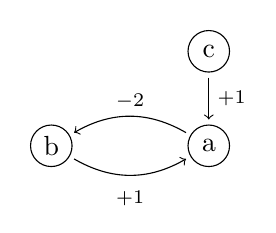
\begin{tikzpicture}[grn]
\path[use as bounding box] (-0.3,-0.75) rectangle (2.5,1.5);
\node[inner sep=0] (a) at (2,0) {a};
\node[inner sep=0] (b) at (0,0) {b};
\node[inner sep=0] (c) at (2,1.2) {c};
%\path
%  node[elabel, below=-1em of a] {$0..2$}
%  node[elabel, below=-1em of b] {$0..1$}
%  node[elabel, below=-1em of c] {$0..1$};
\path[->]
  (b) edge[bend right] node[elabel, below=-2pt] {$+1$} (a)
  (c) edge node[elabel, right=-2pt] {$+1$} (a)
  (a) edge[bend right] node[elabel, above=-5pt] {$-2$} (b);
\end{tikzpicture}
}
\end{minipage}
\begin{minipage}{0.6\linewidth}
\centering
\begin{align*}
K_{a,\{b,c\},\emptyset} &= [2 ; 2] & K_{b,\{a\},\emptyset} &= [0 ; 1] \\
K_{a,\{b\},\{c\}} &= [1 ; 1] & K_{b,\emptyset,\{a\}} &= [0 ; 0] \\
K_{a,\{c\},\{b\}} &= [1 ; 1] &&\\
K_{a,\emptyset,\{b,c\}} &= [0 ; 0] & K_{c,\emptyset,\emptyset} &= [0 ; 1]
\end{align*}
\end{minipage}
\caption{\label{fig:runningBRN}
(left)
IG example.
%Components are represented by nodes labeled with a name and possible expression levels.
Regulations are represented by the edges labeled with their sign and threshold.
For instance, the edge from $b$ to $a$ is labeled $+1$, which stands for: $b \xrightarrow{1} a \in
E_+$.
%and means that if the level of expression of $b$ is equal to (i.e. above) 1, then $b$ activates $a$,
%otherwise, $b$ inhibits $a$.
(right)
Example parametrization of the left IG.
}
\end{figure}

A \emph{state} $s$ of an IG $(\Gamma, E_+, E_-)$ is an element in $\prod_{a \in \Gamma} [0;l_a]$.
$\GRNget{s}{a}$ refers to the level of component $a$ in $s$.
The specificity of Thomas' approach lies in the use of discrete \emph{parameters} to represent the
focal level interval towards which the component will evolve in each configuration of its regulators
(\pref{def:param}).
Indeed, for each possible state of a BRN, all regulators of a component $a$ can be divided into
\emph{activators} and \emph{inhibitors}, given their type of interaction and expression level,
referred to as the \emph{resources} of $a$ in this state (\pref{def:resources}).


\begin{definition}[Discrete parameter $K_{a,A,B}$ and Parametrization $K$]\label{def:param}
For a given component $a \in \Gamma$ and $A$ (resp. $B$) $\subset \GRNreg{a}$ a set of its activators (resp. inhibitors) such that $A \cup B = \GRNreg{a}$ and $A \cap B = \emptyset$,
the discrete \emph{parameter} $K_{a,A,B} = [i; j]$ is a non-empty interval towards which $a$ will tend
in the states where its activators (resp. inhibitors) are the regulators in set $A$ (resp. $B$).
The complete map $K$ of discrete parameters for $\IG$ is called a \emph{parametrization} of $\IG$.
\end{definition}
%A consequence of this definition is that $0 \leq i_1 \leq i_2 \leq l_a$.
%We also denote: $j < K_{a,A,B} \Leftrightarrow j < i_1$ and $j > K_{a,A,B} \Leftrightarrow j> i_2$.

\begin{definition}[Resources $\GRNres{a}{s}$]\label{def:resources}
For a given state $s$ of a BRN, we define the \emph{activators} $A$ and \emph{inhibitors} $B$ of $a$ in $s$ as $\GRNres{a}{s} = A,B$, where:
\begin{align*}
  A &= \{b \in \Gamma \mid \GRNget{s}{b} \in \levelsA{b}{a}\} \\
  B &= \{b \in \Gamma \mid \GRNget{s}{b} \in \levelsI{b}{a}\}
\end{align*}
We also denote: $\GRNallres{a} = \{(A;B) \mid \exists s \in \textstyle\prod_{a \in \Gamma} [0;l_a], \GRNres{a}{s} = A,B\}$
\end{definition}

%\begin{example*}
%\pref{fig:runningBRN}(right) gives a Parametrization of the IG of \pref{fig:runningBRN}(left).
%\end{example*}

At last, \pref{def:dynamics} gives the asynchronous dynamics of a BRN using Thomas' parameters.
From a given state $s$, a transition to another state $s'$ is possible provided that only one component $a$ will evolve of one level towards $K_{a,\GRNres{a}{s}}$.

\begin{definition}[Asynchronous dynamics]\label{def:dynamics}
Let $s$ be a state of a BRN using Thomas' parameters $(\IG, K)$ where $\IG = (\Gamma, E_+, E_-)$.
The state that succeeds to $s$ is given by the indeterministic function $f(s)$:
\begin{align*}
  f(s)  & = s' \Leftrightarrow \exists a \in \Gamma,
    \GRNget{s'}{a} = f^a(s) \wedge
    \forall b \in \Gamma, b \neq a, \GRNget{s}{b} = \GRNget{s'}{b}
    \quad\text{, with}\\
  f^a(s) & =
  \begin{cases}
    \GRNget{s}{a} + 1 & \text{if } \GRNget{s}{a} < K_{a,A,B} \\% \GRNres{a}{s}} \\
    \GRNget{s}{a} & \text{if } \GRNget{s}{a} \in K_{a,A,B} \\ %\GRNres{a}{s}}\\
    \GRNget{s}{a} - 1 & \text{if } \GRNget{s}{a} > K_{a,A,B} % \GRNres{a}{s}}
  \end{cases}
\quad\text{, where $A,B=\GRNres{a}{s}$.}
\end{align*}
\end{definition}

While the use of intervals as parameter values does not add expressivity in boolean
networks, it allows to specify a larger range of dynamics in the general case (w.r.t. the above
definitions).
Indeed, assume that $K_{a,A,B} = [i ; i+2]$;
we aim at obtaining three different parameters $K_{a,A_1,B_1} = i$,  $K_{a,A_2,B_2} = i+1$,
$K_{a,A_3,B_3} = i+2$.
The only possible modification in resources is to add $a$ as a self-regulator.
However, because resources have a boolean definition (a component is either an activator or an inhibitor of
$a$), it is not possible to differentiate the 3 values.
We also remark that the use of intervals makes optional some explicit auto-activations in the IG
(as for $b$ in \pref{fig:runningBRN}, for instance).

\begin{example*}
In the BRN that consists of the IG and parametrization of \pref{fig:runningBRN}, the following
transitions are possible given the semantics defined in \pref{def:dynamics}:
$\GRNetat{a_0, b_1, c_1} \rightarrow \GRNetat{a_1, b_1, c_1} \rightarrow \GRNetat{a_2, b_1, c_1} \rightarrow
\GRNetat{a_2, b_0, c_1} \rightarrow \GRNetat{a_1, b_0, c_1}$,
ending in a steady state,
where $a_i$ is the component $a$ at level $i$.
As $K_{b,\{a\},\emptyset} = [0 ; 1]$, no auto-regulation on $b$ is needed to prevent its evolution when $a$ is not at level $2$.
\end{example*}



% vim:spell spelllang=en:
\section{Interaction Graph Inference from Process Hitting}\label{sec:infer-IG}

The Interaction Graph (IG) is an abstract representation of the direct qualitative influences,
positive and/or negative, between the components of the system.
As discussed in \pref{sec:intro}, the IG allows to efficiently characterize global dynamical
properties for the concrete system, such as the capability for multi-stationarity or oscillation.

In a typical biological network modeling process, a prior IG is generally the starting point for
the formal system specification.
However, it is common that the prior IG actually refers to interactions that reveal to be 
non-effective with respect to the dynamics.
Hence, deriving the IG directly from the dynamical models lead to more concise IGs, enhancing the
conclusiveness of static analyses based upon this abstract representation.

In this section, we formally derive the IG corresponding to a given PH that is well-formed for BRN
modeling.
This section first introduces the notion of focal processes within a PH (\pref{ssec:focal})
which is used to characterize well-formed PH for IG inference (\pref{ssec:wf}).
%and as well used by the parametrization inference presented in \pref{sec:infer-K}.
The rules for inferring the interactions between components from a PH are
described in \pref{ssec:infer-IG}.
We consider hereafter a global PH $(\PHs,\PHl,\PHa)$ on which the IG inference is to be
performed.



\subsection{Focal Processes}\label{ssec:focal}

Many of the inferences defined in the rest of this paper rely on the knowledge of \emph{focal
processes} w.r.t. a given context (a set of processes that are potentially present).
When such a context applies, we expect to (always) reach one focal process in a bounded number of
actions.

For $S_a\subseteq L_a$ and a context (set of processes) $\ctx$, let us define as $\PHa(S_a,\ctx)$
the set of actions on the sort $a$ having their hitter in $\ctx$ and target in $S_a$
(\pref{eq:PHa-ctx});
and the digraph $(V, E)$ where arcs are the bounces within the sort $a$ triggered by actions
in $\PHa(S_a,\ctx)$ (\pref{eq:bounce-graph}).
$\focals(a,S_a,\ctx)$ denotes the set of focal processes of sort $a$ in the scope of
$\PHa(S_a,\ctx)$ (\pref{def:focals}).
\begin{align}
\PHa(S_a,\ctx) & \DEF \{ \PHfrappe{b_i}{a_j}{a_k}\in\PHa \mid b_i\in\ctx \wedge a_j\in S_a \}
\label{eq:PHa-ctx}
\\
\begin{split}
E  & \DEF \{(a_j,a_k)\in (S_a \times \PHl_a) \mid 
			\exists\PHfrappe{b_i}{a_j}{a_k}\in \PHa(S_a,\ctx) \}
\\
V & \DEF S_a \cup \{ a_k\in L_a\mid \exists (a_j,a_k)\in E\}
\end{split}
\label{eq:bounce-graph}
\end{align}

\begin{definition}[$\focals(a,S_a,\ctx)$]\label{def:focals}
The set of processes that are focal for processes in $S_a$ in the scope of $\PHa(S_a,\ctx)$
are given by:
%$\focals(a,S_a,\ctx)$ is the set of focal processes of sort $a$ in the context $\ctx$:
\[
\focals(a,S_a,\ctx) \DEF
\begin{cases}
\{ a_i \in V \mid \nexists (a_i,a_j)\in E\} & \text{if the digraph $(V,E)$ is acyclic},\\
\emptyset & \text{otherwise.}\\
\end{cases}
\]
\end{definition}

We note $\PHl(\ctx)$ the set of states $s\in L$ such that $\forall a\in\PHsort(\ctx), \PHget{s}{a}\in\ctx$,
where $\PHsort(\ctx)$ is the set of sorts with processes in $\ctx$.
We say a sequence of actions $h^1,\dots,h^n$ is \emph{bounce-wise} if and only if
$\forall m\in\segm{1}{n-1}, \PHbounce(h^m)=\PHtarget(h^{m+1})$.
From \pref{def:focals}, it derives that:
\begin{enumerate}
\item if $\focals(a,S_a,\ctx)=\emptyset$, there exists a 
state $s\in \PHl(\ctx\cup S_a)$ such that $\forall n\in\mathbb N$ there
exists a bounce-wise sequence of actions $h^1,\dots,h^{n+1}$ in $\PHa(S_a,\ctx)$ 
with $\PHtarget(h^1)\in s$.
\item if $\focals(a,S_a,\ctx)\neq\emptyset$, for all
state $s\in \PHl(\ctx\cup S_a)$,
for any bounce-wise sequence of actions $h^1,\dots,h^n$ in $\PHa(S_a,\ctx)$ where $\PHtarget(h^1)\in
s$,
either
 $\PHbounce(h^n) \in \focals(a,S_a,\ctx)$,
or
$\exists h^{n+1}\in \PHa(a,\ctx)$ such that $\PHbounce(h^n) = \PHtarget(h^{n+1})$.
Moreover $n\leq|\PHa(S_a,\ctx)|$ (i.e. no cycle of actions possible).
\end{enumerate}

It is worth noticing that those bounce-wise sequences of actions may not be successively playable in
a state $s\in L(\ctx\cup S_a)$.
Indeed, nothing impose that the hitters of actions are present in $s$.
In the general case, the playability of those bounce-wise sequences, referred to as \emph{focals
reachability} may be hard to prove.
However, in the scope of this paper, the particular contexts used with $\focals$ ensure this property.
Notably, the rest of this section uses only \emph{strict} contexts (\pref{def:strict-ctx}) which
allow at most one hitter per sort in the bounce-wise sequences (and thus are present in $s$).

\begin{definition}[Strict context for $S_a$]\label{def:strict-ctx}
A context (set of processes) $\ctx$ is strict for $S_a\subseteq L_a$ if and only if
$\{b_i,b_j\} \subset \ctx \wedge b\neq a \Rightarrow i=j$.
\end{definition}

In other words, assuming focals reachability, if $\focals(a,S_a,\ctx)$ is empty, there exists a
sequence of actions that may be played an unbound number of times (cycle);
if it is non-empty, it is ensured that any state in $\PHl(\ctx\cup S_a)$ converges, in a bounded
number of steps, either to a process in $S_a$ that is not hit by processes in $\ctx$, or to a process in
$L_a\setminus S_a$.

\begin{example}
In the PH of \pref{fig:runningPH-1}, we obtain:
\begin{align*}
\focals(a,L_a,\{b_0,c_0\}) &= \{ a_0 \}
&
\focals(a,L_a,\{b_1,c_1\}) &= \{ a_2 \}
\\
\focals(a,L_a,\{b_1,c_0\}) &= \emptyset
&
\focals(a,\{a_1\},\{b_1,c_0\}) &= \{ a_0, a_2 \}
\end{align*}
\end{example}



\subsection{Well-formed Process Hitting for Interaction Graph Inference}\label{ssec:wf}

The inference of an IG from a PH assumes that the PH defines two types of sorts:
the sorts corresponding to BRN components, and the cooperative sorts.
This leads to the characterization of a \emph{well-formed} PH for IG inference.

The identification of sorts modeling components relies on the observation that their processes
represent (ordered) qualitative levels.
Hence an action on such a sort cannot make it bounce to a process at a distance more than one.
The set of sorts satisfying such a condition is referred to as $\Gamma$
(\pref{eq:PH-components}).
Therefore, in the rest of this paper, $\Gamma$ denotes the set of components of the BRN to infer.

\begin{equation}
\Gamma \DEF \{a \in \PHs \mid \nexists \PHfrappe{b_i}{a_j}{a_k} \in \PHa, |j - k| > 1\} \\
\label{eq:PH-components}
\end{equation}

Any sort that does not act as a component should then be treated as a cooperative sort.
As explained in \pref{ssec:PH}, the role of a cooperative sort $\upsilon$ is to compute the current
state of set of cooperating processes.
Hence, for each sub-state $\sigma$ formed by the sorts hitting $\upsilon$, $\upsilon$ should
converge to a focal process.
This is expressed by \pref{pro:wf-cooperative-sort}, where
the set of sorts having an action on a given sort $a$ is given by 
$\PHdirectpredec{a}$ (\pref{eq:ph_direct_predec})
and $\PHproc(\sigma)$ is the set of processes that compose the sub-state $\sigma$.

\begin{equation}
\forall a \in \PHs, \PHdirectpredec{a} \DEF \{b \in \PHs \mid \exists \PHfrappe{b_i}{a_j}{a_k}\in\PHa \}
\label{eq:ph_direct_predec}
\end{equation}

\begin{property}[Well-formed cooperative sort]\label{pro:wf-cooperative-sort}
A sort $\upsilon\in\PHs$ is a well-formed cooperative sort if and only if
each configuration $\sigma$ of its predecessors leads $\upsilon$ to a unique focal process,
denoted by $\upsilon(\sigma)$:
\[
\forall \sigma \in {\textstyle\prod_{
a\in\PHdirectpredec{\upsilon} \wedge a\neq \upsilon}}
\PHl_{a},
\focals(\upsilon,\PHl_\upsilon,\PHproc(\sigma)\cup \PHl_\upsilon) = \{ \upsilon(\sigma) \}\]
\end{property}

Such a property allows a large variety of definitions of a cooperative sort, but
for the sake of simplicity, does not allow the existence of multiple focal processes.
While this may be easily extended to (the condition becomes 
$\focals(\upsilon,\PHl_\upsilon, \PHproc(\sigma)\cup \PHl_\upsilon)\neq\emptyset$), it makes some
hereafter equations a bit more complex to read as they should handle a set of focal processes instead
of a unique focal process.


Finally, \pref{pro:wf-ph} sums up the conditions for a Process Hitting to be suitable for IG
inference.
In addition of having either component sorts or well-formed cooperative sorts, we also require that
there is no cycle between cooperative sorts, and that
sorts being never hit (\ie{} serving as an invariant environment) are components.

\begin{property}[Well-formed Process Hitting for IG inference]\label{pro:wf-ph}
A PH is well-formed for IG inference if and only if the following conditions are verified:
\begin{itemize}
\item 
each sort $a\in\PHs$ either belongs to $\Gamma$, or is a well-formed cooperative sort;
\item 
there is no cycle between cooperative sorts
(the digraph $(\Sigma,\{(a,b)\in(\Sigma\times\Sigma)\mid \exists \PHfrappe{a_i}{b_j}{b_k}\in\PHa
\wedge a\neq b\wedge \{a,b\}\cap\Gamma=\emptyset \})$ is
acyclic);
\item 
sorts having no action hitting them belong to $\Gamma$
($\{ a \in \Sigma\mid \nexists \PHfrappe{b_i}{a_j}{a_k}\in\PHa\} \subset \Gamma$).
\end{itemize}
\end{property}

\begin{example}
In the PH of \pref{fig:runningPH-2}, $bc$ is a well-formed cooperative sort as defined in \pref{pro:wf-cooperative-sort}, because:
\begin{align*}
\focals(bc, \PHl_{bc}, \{b_0, c_0\} \cup \PHl_{bc}) = \{bc_{00}\} && \focals(bc, \PHl_{bc}, \{b_0, c_1\} \cup \PHl_{bc}) = \{bc_{01}\} \\
\focals(bc, \PHl_{bc}, \{b_1, c_0\} \cup \PHl_{bc}) = \{bc_{10}\} && \focals(bc, \PHl_{bc}, \{b_1, c_1\} \cup \PHl_{bc}) = \{bc_{11}\}
\end{align*}
Hence, both \pref{fig:runningPH-1} and \pref{fig:runningPH-2} are well-formed PH for IG inference
with $\Gamma = \{a,b,c\}$.
\end{example}



\subsection{Interaction Inference}\label{ssec:infer-IG}

At this point we can divide the set of sorts $\PHs$ into components ($\Gamma$, see \pref{eq:PH-components}) and cooperative sorts
($\PHs \setminus \Gamma$) that will not appear in the IG. 
We define in \pref{eq:ph_predec} the set of predecessors of a sort $a$, that is, the sorts influencing $a$
by considering direct actions and possible intermediate cooperative sorts.
The predecessors of $a$ that are components are the regulators of $a$, denoted $\PHpredecgene{a}$
(\pref{eq:regulators}).
\begin{align}
\begin{split}
\forall a \in \PHs, \PHpredec{a} &\DEF \{b \in \PHs \mid \exists n \in \mathbb{N}^*, \exists
(c^k)_{k \in \segm{0}{n}} \in \PHs^{n+1}, \\
                                   & \quad \quad c^0 = b \wedge c^n = a \\
                                   & \quad \quad \wedge \forall k \in \segm{0}{n-1},
                   c^k \in \PHdirectpredec{c^{k+1}} \cap (\PHs\setminus\Gamma)\}
\end{split}
\label{eq:ph_predec}
\\
\forall a\in \PHs, \PHpredecgene{a} & \DEF \PHpredec{a} \cap \Gamma
\label{eq:regulators}
\end{align}

Given a set $g$ of components and a configuration (\ie a sub-state) $\sigma$, $\ctx_g(\sigma)$
refers to the set of processes hitting $a$ regulated by any sort in $g$ (\pref{eq:ctx-sigma}).
If $g=\{b\}$, we simple note $\ctx_b(\sigma)$.
This set is composed of the active processes of sorts in $g$, and the focal process (assumed
unique) of the cooperative sorts $\upsilon$ hitting $a$ that have a predecessor in $g$.
The evaluation of the focal process of $\upsilon$ in context $\sigma$, denoted $\upsilon(\sigma)$,
relies on \pref{pro:wf-cooperative-sort}, which gives its value when all the direct predecessors of
$\upsilon$ are defined in $\sigma$.
When a predecessor $\upsilon'$ is not in $\sigma$, we extend the evaluation by recursively computing
the focal value of $\upsilon'$ is $\sigma$, as stated in \pref{eq:cooperative-eval},
where $\uplus$ stands for a union of states (which are sets of processes).
Because there is no cycle between cooperative sorts, this recursive evaluation of $\upsilon(\sigma)$
always terminates.
\begin{align}
\forall g\subset \Gamma,
  \ctx_g(\sigma) & \DEF \{ \sigma[b] \mid b\in g \} \cup \{ \upsilon(\sigma) \mid
\upsilon\in\PHdirectpredec{a} \setminus \Gamma \wedge g\cap \PHpredecgene{\upsilon} \neq \emptyset \}
\label{eq:ctx-sigma}
\\
\upsilon(\sigma) & \DEF
\upsilon(\sigma \uplus \state{\upsilon'(\sigma) \mid 
  \upsilon'\in\PHdirectpredec{\upsilon} \wedge
  \upsilon'\in\PHs\setminus\Gamma })
\label{eq:cooperative-eval}
\end{align}

This inference mainly focuses on the presence of actions betweens two sorts to conclude on the presence of a regulation.
We aim at inferring that $b$ activates (inhibits) $a$ if there exists a configuration where increasing
the level of $b$ makes possible the increase (decrease) of the level of $a$,
which is directly inspired from the works of~\cite{Richard2010378}.
To do so, the sets of components cooperating together to hit $a$, called groups of influence of $a$, are studied.
Such groups are given by $X(a)$ which is the set of connected components in the graph linking two regulators
$b$ and $c$ of $a$ if they use a common cooperative sort to have an influence on $a$ (\pref{eq:influence-groups}).
\begin{equation}
X(a) = \mathcal C\left( (\PHpredecgene{a}, \{ \{b,c\} \mid
        \exists \upsilon\in \PHdirectpredec{a} \setminus \Gamma,
        \{b,c\} \subset \PHpredecgene{\upsilon} \}) \right)
\label{eq:influence-groups}
\end{equation}

To infer influence of a component $b$ on a component $a$,
we observe the direction of evolution of $a$ for different active processes of $b$.
The fact that $a$ tends to evolve differently when $b$ changes denotes an influence from $b$.
Formally, for a given group $g$ of regulators of a component $a$
(that is, a minimal set of components regulating $a$ through common cooperative sorts),
and a configuration $\ctx$ on $g$, we note
$\irB_a(\sigma)$ the set of processes towards which $a$ can bounce (\pref{eq:possible-bounces}).
%This set is defined using the set $\irF_a(\sigma)$ of action hitting $\PHget{\sigma}{a}$ in $\sigma$ (\pref{eq:possible-actions})
%and the set of processes $\ctx$ hitting any process of $a$ (\pref{eq:ctx-sigma}).
If $a$ cannot be hit by any action in $\sigma$, then $\irB_a(\sigma) = \{ \PHget{\sigma}{a} \}$.
%
\begin{align}
\begin{split}\label{eq:possible-bounces}
  &\forall g \in X(a), \forall \sigma \in \textstyle\prod_{c\in g \cup \{ a \}} \PHl_c,
  \irB_a(\sigma) \DEF 
  \begin{cases}
    \irF_a(\sigma)
      & \text{ if } \irF_a(\sigma) \neq \emptyset\\
    \{ \PHget{\sigma}{a} \}
      & \text{ if } \irF_a(\sigma) = \emptyset
  \end{cases}\\
  &\text{where: } \irF_a(\sigma) \DEF \{ a_k \in \PHl_a \mid \exists b \in \PHs, \exists \PHfrappe{b_i}{a_j}{a_k} \in \PHa,\\
  & \qquad\qquad\qquad\qquad\qquad\qquad \PHget{\sigma}{a} = a_j \wedge \PHget{(\ctx_{g}(\sigma))}{b} = b_i \}\\
\end{split}
\end{align}

\pref{pps:inference-edges} details the inference of all existing influences between components occurring
with a threshold $t$.
The main idea of this inference is that
the presence of a positive (negative) influence of a component $b$ on $a$ denotes the fact that
there exists a state in which increasing the level of $b$ tends to make the future level of $a$ rise (drop)
(\pref{eq:edges-inference}).
Therefore, these influences are split into positive and negative ones, and represent possible edges in the final IG.
Furthermore, studying the influences of the groups of regulators of $a$
allows to study its auto-influences, and thus infer auto-edges on $a$ in the IG (\pref{eq:edges-inference-auto}).
Finally, \pref{eq:edges-inference-noreg} handles the special case where $a$ has no regulators.
We ignore the cases where a component has no visible influence on another.
%
\begin{proposition}[Influences inference]\label{pps:inference-edges}
We define the set of positive (resp. negative) influences $\hat{E}_+$ (resp. $\hat{E}_-$) for any $a\in\Gamma$ by:
\begin{align}
% Arcs a -> b, a ≠ b
\begin{split}\label{eq:edges-inference}
  \forall b\in\PHpredecgene{a}, \forall s \in \{ +, - \}, \\
  b \xrightarrow{t+1} a \in \hat{E}_s \Longleftrightarrow\ & \exists g \in X(a), b \in g,
  \exists \sigma \in \textstyle\prod_{c\in g \cup \{ a \}} \PHl_c, \\
    &\qquad \{ b_t, b_{t+1} \} \subset \PHl_b \wedge b_t \in \sigma,\\
    &\qquad \exists a_j \in \irB_a(\sigma), \exists a_k \in \irB_a(\sigma\{b_{t+1}\}), \\
    &\qquad s = \f{sign}(k - a)
\end{split}\\
% Auto-arcs
\begin{split}\label{eq:edges-inference-auto}
  \forall s \in \{ +, - \}, \quad\qquad\qquad \\
  a \xrightarrow{t+1} a \in \hat{E}_s \Longleftrightarrow\ & \exists g \in X(a), \exists b \in g,
  \exists \sigma \in \textstyle\prod_{c\in g \cup \{ a \}} \PHl_c, \\
    &\qquad \{ b_t, b_{t+1} \} \subset \PHl_b \wedge b_t \in \sigma,\\
    &\qquad \exists a_j \in \irB_a(\sigma), \exists a_k \in \irB_a(\sigma\{b_{t+1}\}), \\
    &\qquad s = \f{sign}(a_k - a_j)
\end{split}\\
\begin{split}\label{eq:edges-inference-noreg}
  \forall s \in \{ +, - \}, \quad\qquad\qquad \\
  a \xrightarrow{t+1} a \in \hat{E}_s \Longleftrightarrow\ & \reg{a} = \emptyset \wedge \{ a_t, a_{t+1} \} \subset \PHl_a, \\
    &\qquad \exists a_j \in \irB_a(\PHetat{a_t}), \exists a_k \in \irB_a(\PHetat{a_{t+1}}), \\
    &\qquad s = \f{sign}(a_k - a_j)
\end{split}
\end{align}
where $\f{sign}(x) = \begin{cases}|x|/x & \text{ if $x \neq 0$} \\ 0 & \text{ if $x = 0$}\end{cases}$.
\end{proposition}

We are now able to infer the edges of the final IG by considering positive and negative influences
(\pref{pps:inference-IG}).
We infer a positive (resp. negative) edge if there only exist corresponding influences with the same sign.
If an influence is both positive and negative, we infer an unsigned edge.
In the end, the threshold of each edge is the minimum threshold for which an influence has been found.
%
\begin{proposition}[Interaction Graph inference]\label{pps:inference-IG}
We infer $\IG = (\Gamma,E)$ using \pref{pps:inference-edges} as follows:
\begin{align*}
E_+ &= \{ \GRNedge{a}{+}{t}{b} \mid \nexists a \xrightarrow{t'} b \in \hat{E}_-
  \wedge t = \min \{ l \mid a \xrightarrow{l} b \in \hat{E}_+\}\} \\
E_- &= \{ \GRNedge{a}{-}{t}{b} \mid \nexists a \xrightarrow{t'} b \in \hat{E}_+
  \wedge t = \min \{l \mid a \xrightarrow{l} b \in \hat{E}_-\}\} \\
E_\pm &= \{ \GRNedge{a}{\uns}{t}{b} \mid \exists a \xrightarrow{t'} b \in \hat{E}_+ \wedge \exists a \xrightarrow{t''} b \in \hat{E}_- \\
  & \qquad\qquad\qquad \wedge t = \min \{l \mid a \xrightarrow{l} b \in \hat{E}_- \cup \hat{E}_+\}\}
\end{align*}
\end{proposition}



\begin{example}
The IG inference of the PH of \pref{fig:runningPH-1} gives the
IG in \pref{fig:BRN-inf1}, containing the following edges:
\begin{align*}
  E_+ &= \{\GRNedgef{b}{+}{1}{a}, \GRNedgef{c}{+}{1}{a}, \GRNedgef{a}{+}{1}{a}, \GRNedgef{b}{+}{1}{b}, \GRNedgef{c}{+}{1}{c}\}\\
  E_- &= \{\GRNedgef{a}{-}{2}{b}\} \qquad\qquad\qquad\qquad\qquad
  E_\uns = \emptyset
\end{align*}
This IG is close to the one in \pref{fig:runningBRN} but not equivalent,
as each component has an additional auto-action.
The auto-actions on $b$ and $c$ are the consequence of a global stability
in some configurations: $c$ never evolves, and neither does $b$ when $a_2$ is not active.
The auto-action on $a$ is mainly caused by its multi-valued nature.

The inference of the refined PH of \pref{fig:runningPH-2} gives the same IG.

\begin{figure}[t]
\centering
\scalebox{1.2}{
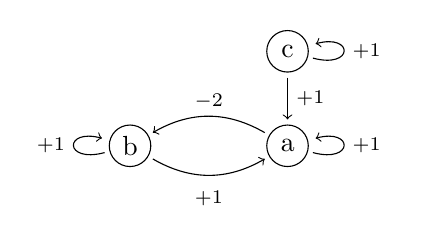
\begin{tikzpicture}[grn]
  \path[use as bounding box] (-1.3,-0.75) rectangle (3.5,1.5);
  \node[inner sep=0] (a) at (2,0) {a};
  \node[inner sep=0] (b) at (0,0) {b};
  \node[inner sep=0] (c) at (2,1.2) {c};
  \path[->]
    (b) edge[bend right] node[elabel, below=-2pt] {$+1$} (a)
    (c) edge node[elabel, right=-2pt] {$+1$} (a)
    (a) edge[bend right] node[elabel, above=-5pt] {$-2$} (b)
    (b) edge[in=-15+180, out=15+180, loop] node[elabel, left=-2pt] {+1} (b)
    (c) edge[in=15, out=-15, loop] node[elabel, right=-2pt] {+1} (c)
    (a) edge[in=15, out=-15, loop] node[elabel, right=-2pt] {+1} (a);
\end{tikzpicture}
}
\caption{\label{fig:BRN-inf1}
  Result of the IG inference performed on the PH of \pref{fig:runningPH-2}.
}
\end{figure}

\end{example}



\begin{example}
If we add the action $\PHfrappe{a_2}{b_0}{b_1}$ to the PH of \pref{fig:runningPH-2},
then two unsigned edges towards $b$ are inferred instead of the previous signed edges:
\begin{align*}
  E_+ &= \{\GRNedgef{b}{+}{1}{a}, \GRNedgef{c}{+}{1}{a}, \GRNedgef{a}{+}{1}{a}, \GRNedgef{c}{+}{1}{c}\}\\
  E_- &= \emptyset \qquad\qquad\qquad\qquad
  E_\uns = \{\GRNedgef{a}{\uns}{2}{b}, \GRNedgef{b}{\uns}{1}{b}\}
\end{align*}
This is due to the fact that the actions $\PHfrappe{a_2}{b_1}{b_0}$ and $\PHfrappe{a_2}{b_0}{b_1}$
introduce an oscillation only caused by $a$, which cannot be represented in Thomas modeling.
\end{example}

\section{Parametrization inference}\label{sec:infer-K}

Given the IG inferred from a PH as presented in the previous section, one can find the discrete parameters that model the behavior of the studied PH using the method presented in the following.
It relies on an exhaustive enumeration of all predecessors of each component in order to find attractor processes and returns a possibly incomplete parametrization, given the exhaustiveness of the cooperations.
The last step consists of the enumeration of all compatible complete parametrizations given this
set of inferred parameters, the PH dynamics and some biological constraints on parameters.

\subsection{Parameters inference}

\todo{Try to address the inference of parameters despite unsigned edges}

This subsection presents some results related to the inference of independent discrete parameters from a given PH.
These results are equivalent to those presented in \cite{PMR10-TCSB}, with notation adapted to be shared with the previous section.
In addition, we introduce the well-formed PH for parameter inference property (\pref{pro:wf-ph-K}),
which implies that the inferred IG does not contain any unsigned interactions, and thus can be seen as the
regular IG $(\Gamma, E)$,
and that any processes in $\levels{b}{a}$ (resp. $\ulevels{b}{a}$) share the same behavior
regarding $a$.

\new{Changed $\levelsA{a}{b}$ and $\levelsI{a}{b}$ into $\levels{a}{b}$ in \pref{eq:wf-levels} and \pref{eq:param_context}.}

\begin{property}[Well-formed PH for parameter inference]\label{pro:wf-ph-K}
A PH is well-formed for parameter inference if and only if
it is well-formed for IG inference, and
the IG $(\Gamma, E)$ inferred by \pref{pps:inference-IG}
verifies the following property:
\begin{align}
\begin{split}
\forall b\in \GRNreg{a} &,
	\forall (i,j\in\levels{b}{a} \vee i,j\in\ulevels{b}{a}), \\
& \qquad \forall c \in \Gamma, ( (b\neq a\wedge c=a) \vee (c\in\PHpredec{a} \wedge b\in\PHdirectpredec{c})), \\
& \qquad \qquad
			\PHfrappe{b_i}{c_k}{c_l}\in\PHa \Leftrightarrow
				\PHfrappe{b_j}{c_k}{c_l}\in\PHa
\end{split}
\label{eq:wf-levels}
\end{align}
\end{property}

Let $K_{a,\omega}$ be the parameter we want to infer for a given component $a \in \Gamma$
%and $A,B \in \GRNallres{a}$ a configuration of resources of $a$ (activators and inhibitors).
and $\omega \subset \GRNreg{a}$ a set of its regulators.
This inference, as for the IG inference, relies on the search of focal processes of the component for the given configuration of its regulators.

For each sort $b \in \GRNreg{a}$, we define a context $C^b_{a,\omega}$ in \pref{eq:param_context} that contains all processes representing the influence of the resources in the configuration modeled by $\omega$.
The context of a cooperative sort $\upsilon$ that regulates $a$ is given in
\pref{eq:param_context_coop} as the set of focal processes matching the current configuration.
$C_{a,\omega}$ refers to the union of all these contexts (\pref{eq:K-ctx}).
\begin{align}
\label{eq:param_context}
\forall b\in\Gamma,~
C_{a,\omega}^b & \DEF \begin{cases}
  \levels{b}{a} & \text{if $b \in \omega$,}\\
  \ulevels{b}{a} & \text{if $b \notin \omega$,}\\
  L_b            & \text{otherwise;}\\
\end{cases}
\\
\label{eq:param_context_coop}
\forall \upsilon \in \PHpredec{a}\setminus\Gamma,~
C_{a,\omega}^\upsilon & \DEF \{
\upsilon(\sigma) \mid \sigma \in \textstyle\prod_{c\in\PHdirectpredec{\upsilon}}C_{a,\omega}^c \}
\\
C_{a,\omega} & \DEF \textstyle\bigcup_{b\in\PHpredec{a}} C^b_{a,\omega}
\label{eq:K-ctx}
\end{align}

The parameter $K_{a,\omega}$ specifies to which values $a$ eventually evolves as long as the context
$C_{a,\omega}$ holds, which is precisely the definition of the $\focals$ function
(\pref{def:focals} in \pref{ssec:focal}),
where the focals reachability property can be derived from \pref{pro:wf-ph-K} and
\pref{eq:param_context_coop}.
Hence $K_{a,\omega} = \focals(a,C^a_{a,\omega},C_{a,\omega})$ if this latter is a non-empty interval
(\pref{pps:param_K}).

\begin{proposition}[Parameter inference]
\label{pps:param_K}
Let $(\PHs, \PHl, \PHh)$ be a Process Hitting well-formed for parameter inference, and $\IG = (\Gamma, E)$ the inferred IG.
Let $A$ (resp. $B$) $\subseteq \Gamma$ be the set of regulators that activate (resp. inhibit) a sort
$a$.
%If $\focals(a,C_{a,A,B})$ is a non-empty interval, then $K_{a,A,B} = \focals(a, C_{a,A,B})$.
If $\focals(a,C^a_{a,\omega},C_{a,\omega})=[a_i;a_j]$ is a non-empty interval, 
	then $K_{a,\omega} = [i;j]$.
\end{proposition}

\begin{example*}
Applied to the PH in \pref{fig:runningPH-1}, we obtain, for instance, 
$K_{b,\emptyset} = [0 ; 1]$ and
$K_{a,\{b,c\}} = [2 ; 2]$,
while $K_{a,\{b\}}$ can not be inferred.
For the PH in \pref{fig:runningPH-2}, this latter is evaluated to $[1;1]$.
\end{example*}

Given the \pref{pps:param_K}, we see that in some cases, the inference of the targeted parameter is impossible.
This can be due to a lack of cooperation between regulators: when two regulators independently hit a component, their actions can have opposite effects, leading to either an indeterministic evolution or to oscillations.
Such an indeterminism is not possible in a BRN as in a given configuration of regulators, a component can only have an interval attractor, and eventually reaches a steady-state.
In order to avoid such inconclusive cases, one has to ensure that no such behavior is allowed by
either removing undesired actions or using cooperative sorts to prevent opposite influences between
regulators.

\subsection{Admissible parametrizations}\label{ssec:admissible-K}

When building a BRN, one has to find the parametrization that best describes the desired behavior of the studied system.
Complexity is inherent to this process as the number of possible parametrizations for a given IG is exponential w.r.t. the number of components.
However, the method of parameters inference presented in this section gives some information about necessary parameters given a certain dynamics described by a PH.
This information thus drops the number of possible parametrizations, allowing to find the desired behavior more easily.

We first delimit the validity of a parameter (\pref{pro:K-valid}) in order to ensure that any
transition in the resulting BRN is allowed by the studied PH.
This is verified by the existence of a hit making the concerned component bounce into the direction
of the value of the parameter in the matching context.
Thus, assuming \pref{pro:wf-ph-K} holds, any transition in the inferred BRN corresponds to at least
one transition in the PH, proving the correctness of our inference.
We remark that any parameter inferred by \pref{pps:param_K} satisfies this property.

\new{Update all assumptions.}

\begin{property}[Parameter validity]\label{pro:K-valid}
A parameter $K_{a,\omega}$ is valid w.r.t. the PH iff the following equation is verified:
\begin{align*}
\forall a_i\in C^a_{a,\omega},
		a_i \notin K_{a,\omega} \Longrightarrow (
  \exists \PHfrappe{c_k}{a_i}{a_j}\in\PHa, & c_k \in C^c_{a,\omega} \\
 \wedge a_i < K_{a,\omega} \Rightarrow j > i 
 & \wedge  a_i > K_{a,\omega} \Rightarrow j <i )
\end{align*}
\end{property}
		

Then, we use some additional biological constraints on Thomas' parameters given in
\cite{BernotSemBRN}, that we sum up in the following three properties:

\begin{property}[Extreme values assumption]
Let $\IG = (\Gamma, E)$ be an IG. A parametrization $K$ on $\IG$ satisfies the \emph{extreme values assumption} iff:
\label{prop:param_enum_extreme}
\[
  \forall b \in \Gamma, \GRNreg{b} \neq \emptyset \Longrightarrow \exists \omega \subset \GRNreg{b}, 0 \in K_{b,\omega} \wedge \exists \omega' \subset \GRNreg{b}, l_b \in K_{b,\omega'}
\]
\end{property}

\begin{property}[Activity assumption]
\label{prop:param_enum_activity}
Let $\IG = (\Gamma, E)$ be an IG. A parametrization $K$ on $\IG$ satisfies the \emph{activity assumption} iff:
\begin{align*}
%  \forall b \in \Gamma, \forall a \in \GRNreg{b}, \exists (A;B) \in \GRNallres{a}, K_{b,A,B} <_{[]} K_{b,A \cup \{b\},B \setminus \{b\}}
%\\
%  \forall b \in \Gamma, \forall a \in \GRNreg{b}, \exists (A;B) \in \GRNallres{a}, K_{b,A \setminus \{b\},B \cup \{b\}} <_{[]} K_{b,A,B}
  \forall b \in \Gamma, \forall a \in \GRNreg{b}, \exists \omega \subset \GRNreg{b}, K_{b,\omega} \neq K_{b,\omega \cup \{ a \}}
\end{align*}
\end{property}

\begin{property}[Monotonicity assumption]
\label{prop:param_enum_monotonicity}
Let $\IG = (\Gamma, E)$ be an IG. A parametrization $K$ on $\IG$ satisfies the \emph{monotonicity assumption} iff:
%\[
%  \forall b \in \Gamma, \forall (A;B), (A';B') \in \GRNallres{b},
%  A \subset A' \wedge B' \subset B \Rightarrow K_{b,A,B} \leq_{[]} K_{b,A',B'}
%\]
$\forall b \in \Gamma$,
$\forall X^+ \subset \{ a \in \Gamma \mid \GRNedge{a}{+}{t}{b} \in E_+ \}$,
$\forall X^- \subset \{ a \in \Gamma \mid \GRNedge{a}{-}{t}{b} \in E_- \}$,
%A \subset A' \wedge B' \subset B \Rightarrow
$K_{b,\omega \cup X^-} \leq_{[]} K_{b,\omega \cup X^+}$
\end{property}

\begin{comment}
\begin{definition}[Admissible parametrization \& Admissible parametrization with respect to inferred parameters]
\label{def:param_enum_inf}
Let $\PH = (\PHs, \PHl, \PHh)$ be a PH so that IG inference is possible, and $\IG = (\Gamma, E_+,
E_-)$ the inferred IG.
A parametrization $K$ on $\IG$ is said to be \emph{admissible} iff it respects
the extreme values assumption, the activity assumption and the monotonicity assumption.
A parametrization $K$ on $\IG$ is said to be \emph{admissible with respect to the
inferred parameters} iff it is admissible and that all parameters that can be inferred regarding
\pref{pps:param_K} are equal to their inferred value.
\end{definition}

\todo{utilité de “Admissible parametrization” seul ?}
\end{comment}


\subsection{Answer Set Programming implementation concepts}

\rewrite{This whole subsection may be completed, or turned into a new section}

\todo{Rewrite implementation with the new semantics}

\newcommand{\ti}[1]{\texttt{\textit{#1}}}
\newcommand{\aspil}[1]{\texttt{#1}}
\newcommand{\asp}[1]{\begin{itemize} \item[] \aspil{#1} \end{itemize}}

Answer Set Programming (ASP) \cite{Baral03} has been chosen to address the enumeration of all admissible parametrizations.
The motivations are following:
\begin{itemize}
  \item ASP efficiently tackles the inherent complexity of the models we use, thus allowing a fast execution of the formal tools defined in this paper,
  \item it is convenient to enumerate a large set of possible answers,
  \item it allows us to easily constrain the answers according to some properties.
\end{itemize}
We now synthesize some key points to better make the reader understand our ASP implementation with the enumeration example.

All information describing the studied model (PH and inferred IG \& parameters) are expressed in ASP using facts.
For functional purposes, we assign a unique label to each couple $A,B$ of activators and inhibitors of a given component, and in the following we note $K^p_{a,A,B}$ the parameter of component $a$ whose regulators $A,B$ are assigned to the label $p$.
Then, to state the existence of a parameter $K^\ti{p}_{\ti{a},A,B}$, we use an atom named \aspil{param\_label} in the following fact:
\asp{param\_label(\ti{a}, \ti{p}).}

Defining a set in ASP is equivalent to defining the rule for belonging to this set.
For example, we define an atom \aspil{param\_act} that describes the set of active regulators of a given a parameter.
%of component \ti{a} and label \ti{p} (\ie the set $A$ of a parameter $K^\ti{p}_{\ti{a},A,B}$).
Describing the activators of $K^\ti{p}_{\ti{a},\{\ti{b},\ti{c}\},\{\ti{d}\}}$ gives:
\asp{param\_act(\ti{a}, \ti{p}, \ti{b}).
\item[] param\_act(\ti{a}, \ti{p}, \ti{c}).}
The absence of such a fact involving \ti{d} with label \ti{p} indicates that \ti{d} is an inhibitor in the configuration of regulators related to this parameter.

Rules allow more detailed declarations than facts as they have a body (right-hand part below) containing constraints and allowing to use variables, while facts only have a head (left-hand part).
For instance, in order to define the set of expression levels of a component, we declare:
\asp{component\_levels(X, 0..M) :- component(X, M).}
where the \aspil{component(X, M)} atom stands for the existence of a component \aspil{X} with a maximum level \aspil{M}.
Considering this declaration, any possible answer for the atom \aspil{component\_levels} will be found by binding all possible values of its two terms with all existing \aspil{component} facts: the existence of an answer \aspil{component\_levels(\ti{a}, \ti{k})} will depend on the existence of a term \ti{a}, which is bound with \aspil{X}, and an integer~\ti{k}, constrained by: $0 \leq \ti{k} \leq \aspil{M}$.

Cardinalities are convenient to enumerate all possible parametrizations by creating multiple answer sets.
A cardinality (denoted hereafter with curly brackets) gives any number of possible answers for some atoms between a lower and upper bounds.
For example,
\asp{1 \{ param(X, P, I) : component\_levels(X, I) \} :-
\item[] ~~~~~~param\_label(X, P), not infered\_param(X, P).}
where \aspil{param(X, P, I)} stands for: $\aspil{I} \in K^\aspil{P}_{\aspil{X},A,B}$,
means that any parameter of component \aspil{X} and label \aspil{P} must contain at least one level value (\aspil{I}) in the possible expression levels of \aspil{X}.
Indeed, the lower bound is 1, forcing at least one element in the parameter, but no upper bound is specified, allowing up to any number of answers.
The body (right-hand side) of the rule also checks for the existence of a parameter of \aspil{X} with label \aspil{P}, and constrains that the parametrization inference was not conclusive for the considered parameter (\aspil{not} stands for negation by failure: \aspil{not L} becomes true if \aspil{L} is not true).
Such a constraint gives multiple results as any set of \aspil{param} atoms satisfying the cardinality will lead to a new global set of answers.
In this way, we enumerate all possible parametrizations which respects the results of parameters
inference, but completely disregarding the notion of admissible parametrizations given in
\pref{ssec:admissible-K}.

We rely on integrity constraints to filter only admissible parametrizations.
An integrity constraint is a rule with no head, that makes an answer set unsatisfiable if its body turns out to be true.
Hence, if we suppose that:
\begin{itemize}
  \item the \aspil{less\_active(\ti{a}, \ti{p}, \ti{q})} atom means that $K^\ti{p}_{\ti{a},A,B}$ stands for a configuration with less activating regulators than $K^\ti{q}_{\ti{a},A',B'}$ (\ie $A \subset A'$),
  \item the \aspil{param\_inf(\ti{a}, \ti{p}, \ti{q})} atom means: $K^\ti{p}_{\ti{a},A,B} \leq_{[]} K^\ti{q}_{\ti{a},A',B'}$,
\end{itemize}
the monotonicity assumption is formulated as the following integrity constraint:
\asp{:- less\_active(X, P, Q), not param\_inf(X, P, Q).}
which removes all parametrization results where parameters $K^\aspil{P}_{\aspil{X},A,B}$ and $K^\aspil{Q}_{\aspil{X},A',B'}$ exist such that $A \subset A'$ and $K^\aspil{Q}_{\aspil{X},A',B'} <_{[]} K^\aspil{P}_{\aspil{X},A,B}$, thus violating the monotonicity assumption.
Of course, other assumptions can be formulated in the same way.

This subsection succinctly described how we write ASP programs to represent a model and solve all steps of Thomas' modeling inference.
It finds a particularly interesting application in the enumeration of parameters: all possible parametrizations are generated in separate answer sets, and integrity constraints are formulated to remove those that do not fit the assumptions of admissible parametrizations,
thus reducing the number of interesting parametrizations to be considered in the end.

\section{Answer Set Programming implementation concepts}\label{sec:impl}

\todo{Proofread this whole section}

\newcommand{\ti}[1]{\texttt{\textit{#1}}}
\newcommand{\aspil}[1]{\texttt{#1}}
\newcommand{\asp}[1]{\begin{itemize} \item[] \aspil{#1} \end{itemize}}

%\newcommand{\atom}{\mathbf}
\newcommand{\atom}[1]{#1}
%\newcommand{\predicate}{\mathbf}
\newcommand{\predicate}[1]{#1}
\newcommand{\la}{\leftarrow}
\newcommand{\var}[1]{#1}
\newcommand{\nota}{\neg}

\newcommand{\paramlabel}{\predicate{param\_label}}
\newcommand{\paramres}{\predicate{param\_resource}}
\newcommand{\component}{\predicate{component}}
\newcommand{\componentlevels}{\predicate{component\_levels}}
\newcommand{\param}{\predicate{param}}
\newcommand{\inferedparam}{\predicate{infered\_param}}
\newcommand{\lessactive}{\predicate{less\_active}}
\newcommand{\paraminf}{\predicate{param\_inf}}



Answer Set Programming (ASP) is a logic programming paradigm \cite{Baral03},
which has been chosen to address the enumeration of all admissible parametrizations.
The motivations are following:
\begin{itemize}
  \item ASP efficiently tackles the inherent complexity of the models used, thus allowing a fast execution of the formal tools defined in this paper,
  \item it is convenient to enumerate a large set of possible answers,
  \item and it allows to easily constrain the answers according to some properties.
\end{itemize}
We now synthesize some key points to better make the reader understand our ASP implementation with the enumeration example.

\subsection{Simple rules}\label{sssec:simple_rules}
ASP is based on a set of rules of of the form:
\begin{align*}
  \underbrace{{\ }\atom{H}_{\ }}_{head} \la \underbrace{\atom{A}_1, \atom{A}_2, \dots, \atom{A}_n, \nota \atom{B}_1, \nota \atom{B}_2, \dots, \nota \atom{B}_m}_{body}.
\end{align*}
where the $body$ is a series of atoms ($\atom{A}_i$) and negations of atoms ($\nota \atom{B}_i$).
In the case of \emph{simple rules} (as opposed to the \emph{cardinality rules} of \pref{sssec:cardinality_rules}), the $head$ is also an atom ($\atom{H}$).
Such a rule states that if all atoms $\atom{A}_1, \atom{A}_2, \dots, \atom{A}_n$ are true
and all atoms $\atom{B}_1, \atom{B}_2, \dots, \atom{B}_m$ are not true (negation by failure), then $\atom{H}$ has to be true.
Solving an ASP program means finding an \emph{answer set}, that is a minimal set of true atoms that respect all the rules.
Several answer sets can be solution to the same ASP program and the solver can be directed to enumerate them all.

An atom is composed of a predicate and a series of arguments (possibly empty).
For example, the following atom:
\begin{align*}
  \predicate{p}(x_1, x_2, \dots, x_r)
\end{align*}
is composed of the predicate $\predicate{p}$ and $r$ arguments: $x_1, x_2, \dots, x_r$.
Each argument can be either an constant or a variable, %value -> constant
a constant being a representation of a piece of data (component name, expression level, …)
and a variable is used to represent any possible existing constant which respects the rules.
In this paper, a variable is always denoted by a single capital letter (e.g.~$\var{A}$, $\var{P}$, $\var{Q}$, …)
while constants are either numerical or consist of a single lowercase letter (e.g.~$a$, $b$, $c$, $1$, $2$, …).

A rule with no $body$ part is called a fact, and its $head$ atom has to belong to all answer sets.
For instance, the information describing the studied model (the original PH model and the inferred IG and parameters) are expressed in ASP using facts.
In particular, the predicate $\component$ allows to define all components belonging to the inferred IG.
Thus, an atom $\component(a, m)$ states that $a$ is a component of the IG and that $l_a = m$.

\begin{example}
Consider \pref{ex:infer-param-runningPH-1}: the inferred IG contains 3 components, and to state the existence of each of them, the following facts are used:
\begin{align*}
  &\component(a, 2). \\
  &\component(b, 1). \\
  &\component(c, 1).
\end{align*}
These three atoms are built with the predicate $\component$.
Furthermore, $a$, $b$, $c$, $1$ and $2$ are constants.
\end{example}

To describe the sets of all expression levels of each component (\ie the set $\segm{0}{l_a}$ for each $a \in \Gamma$),
one can use atoms of the form $\componentlevels(a, k)$ to state that $k \in \segm{0}{l_a}$.
Variables here come in handy to enumerate each possible constant $k$ for each component $a$:
during the solving, any rule containing variables is duplicated in order to replace each variable by all the possible constants it could represent.
The following rule, for example, contains three variables ($\var{A}$, $\var{K}$ and $\var{M}$) and enumerates the set of possible expression levels of each component in the system:
\begin{align*}
  \componentlevels(A, K) \la \component(\var{A}, \var{M}), 0 \leq K \leq M.
\end{align*}
where the notation “$\leq$” stands for a shortcut in ASP which has the same meaning as the mathematical operator.

\begin{example}
Regarding \pref{ex:infer-param-runningPH-1}, the previous rule will make the following set of atoms belong to every answer set:
\begin{align*}
  &\{&&\componentlevels(b, 0),
  &&\componentlevels(b, 1), \\
  &&&\componentlevels(c, 0),
  &&\componentlevels(c, 1), \\
  &&&\componentlevels(a, 0),
  &&\componentlevels(a, 1), \\
  &&&\componentlevels(a, 2) &&&&\}
\end{align*}
\end{example}

\subsection{Cardinality rules}
\label{sssec:cardinality_rules}
As an extension of simple rules, \emph{cardinality rules} turn out to be convenient to enumerate a set of answer sets.
The head of a cardinality rule specifies a set of atoms $H$ and two integers $min$ and $max$, and is denoted:
\begin{align*}
  min\ \{\ H\ \}\ max \la \atom{A}_1, \atom{A}_2, \dots, \atom{A}_n, \nota \atom{B}_1, \nota \atom{B}_2, \dots, \nota \atom{B}_m.
\end{align*}
Given such a rule, as many answer sets as possible are created, so that each answer set $S$ verifies:
\begin{align*}
  min \leq |S \cap H| \leq max
\end{align*}
and every atom $\atom{H}_i \in S \cap H$ respects the simple rule:
\begin{align*}
  \atom{H}_i \la \atom{A}_1, \atom{A}_2, \dots, \atom{A}_n, \nota \atom{B}_1, \nota \atom{B}_2, \dots, \nota \atom{B}_m.
\end{align*}
In other words, all answer sets contain a subset of $H$ whose cardinality goes from $min$ to $max$.
The set of atoms $H = \{ \atom{H}_1, \atom{H}_2, \dots, \atom{H}_p \}$ is often defined as: $H = \atom{P} \mid \atom{Q}$,
which is a shorthand for “the set of atoms of the form $\atom{P}$ for which $\atom{Q}$ is true”.
%\rewrite{Reformulate?}

Cardinality rules turn out to be convenient to enumerate all possible parametrizations by creating multiple answer sets.
For functional purposes, a unique label is assigned to every possible set of resources of a given component.
Thus, we denote $\omega_p$ the set of resources of a given component $a$ labeled by $p$,
and naturally, $K_{a,\omega_p}$ is the related parameter.
%and in the following we note $K_{a,\omega_p}$ the parameter of component $a$ whose set of resources $\omega$ is assigned to the label $p$.
We note that labeling the sets of resources of a component is obviously equivalent to labeling its parameters.
Then, suppose that:
\begin{itemize}
  \item $\paramlabel(a, p)$ states that $p$ is a valid label for a set of resources of component $a$ (and therefore $K_{a,\omega_p}$ is a valid parameter);
  \item $\param(a, p, i)$ states that: $i \in K_{a, \omega_p}$;
  \item $\inferedparam(a, p)$ states that the parameter inference of $K_{a, \omega_p}$ was conclusive (\pref{pps:param_K}).
\end{itemize}
It is thereby possible to enumerate the possible values of all parameters for which \pref{pps:param_K} was not conclusive, with the following cardinality rule:
\begin{align*}
  & 1\ \{\ \param(\var{A}, \var{P}, \var{I}) \mid \componentlevels(\var{A}, \var{I})\ \}\ \infty\ \la \\
  & \qquad\qquad\qquad \paramlabel(\var{A}, \var{P}), \nota \inferedparam(\var{A}, \var{P}).
\end{align*}
Indeed, this rule applies to any possible parameter $\var{P}$ of any component $\var{A}$ ($\paramlabel$) whose value is still unknown ($\nota \inferedparam$),
and states that any expression level $\var{I}$ of this component ($\componentlevels$) can belong to the value of the parameter ($\param$).
Furthermore, the lower bound is $1$, which forces each enumerated parameter to contain at least one value,
but no upper bound is specified ($\infty$) for the size of each parameter
(which is already bounded by the number of possible expression levels of the related component).
%each parameter contains at least $1$ value, as stated by the lower bound, and has no upper bound ($\infty$) but the number of expression levels of its component.
In other worlds, this cardinality rule creates as many answer sets as there are \emph{candidate} parametrizations
so that if $K_{a, \omega_p}$ could not be inferred by \pref{pps:param_K}, then
$K_{a, \omega_p} \subset \segm{0}{l_a} \wedge K_{a, \omega_p} \neq \emptyset$
(thus completely disregarding the notion of admissible parametrizations given in \pref{ssec:admissible-K} or the fact that parameters have to be intervals).


%so that
%inferred parameters with \pref{pps:param_K} keep their value and
%parameters that could not be inferred take any possible value amongst the expression levels of the related component: $K_{a, \omega_p} \subset \segm{0}{l_a} \wedge K_{a, \omega_p} \neq \emptyset$.

\begin{example}\label{ex:cardinality}
In the scope of \pref{ex:infer-param-runningPH-1}, $K_{a,\{a,b\}}$ and $K_{a,\{a,c\}}$ could not be inferred by \pref{pps:param_K}.
The previous cardinality rule allows to produce 49 parametrizations, in which these two parameters can take all possible values:
%The enumeration thus produces 36 parametrizations, in which these parameters can take all possible values:
%(as, in this case, the assumptions of \pref{ssec:admissible-K} bring no new constraint):
\begin{align*}
  (K_{a,\{a,b\}} ; K_{a,\{a,c\}}) \in \{ \segm{0}{0} , \segm{1}{1} , \segm{2}{2} , \segm{0}{1} , \segm{1}{2} , \segm{0}{2}, \{ 0, 2 \} \}^2
\end{align*}
and all the other parameters keep their inferred values.
%These parametrizations take the form of sets of $\param$ atoms.
Note that $\{ 0, 2 \}$ belongs to the set of candidate parametrizations
as no rule specifying that a parameter has to be an interval has been defined yet.
\end{example}



\subsection{Constraints}\label{sssec:constraints}
%Finally, constraints can be used to filter answer sets that model parametrizations which are impossible or do not respect the assumptions of \pref{ssec:admissible-K}.
Finally, a constraint is a rule with no $head$ part:
\begin{align*}
  \la \atom{A}_1, \atom{A}_2, \dots, \atom{A}_n, \nota \atom{B}_1, \nota \atom{B}_2, \dots, \nota \atom{B}_m.
\end{align*}
A constraint is satisfied only if its $body$ is not satisfied,
which thus allows to invalidate answer sets containing some unwanted combinations of atoms.
In the scope of parameters enumeration, for example, constraints are especially useful to filter parametrizations
that contain non-interval parameters, or that do not respect the assumptions of \pref{ssec:admissible-K}.
Indeed, suppose that:
\begin{itemize}
  \item $\lessactive(a, p, q)$ states that $\omega_p$ is a set of resources of $a$ with (loosely) less activators and more inhibitors than $\omega_q$;
  \item $\paraminf(a, p, q)$ states that: $K_{a,\omega_p} \leqsegm K_{a,\omega_q}$.
\end{itemize}
Then, the monotonicity assumption (\pref{pro:param_enum_monotonicity}) is formulated as the following constraint:
\begin{align*}
  \la \lessactive(\var{A}, \var{P}, \var{Q}), \nota \paraminf(\var{A}, \var{P}, \var{Q}).
\end{align*}
Indeed, this constraint removes all parametrization results where parameters $K_{\var{A},\omega_\var{P}}$ and $K_{\var{A},\omega_\var{Q}}$ exist
such that $\var{A}$ is less activated by the set of resources $\omega_\var{P}$ than it is by $\omega_\var{Q}$,
but $K_{\var{A},\omega_\var{Q}} \ltsegm K_{\var{A},\omega_\var{P}}$,
thus violating the monotonicity assumption.
Of course, other assumptions can be formulated in the same way.

\begin{example}

The set of candidate values given in \pref{ex:cardinality} can be filtered using constraints.
For example, a constraint was written in order to obtain only interval parameter
(thus avoiding parameters with “gaps” such as $\{ 0, 2 \}$).
Applying such a constraint would reduce the set of possible values for the parameters $K_{a,\{a,b\}}$ and $K_{a,\{a,c\}}$ to:
\begin{align*}
  (K_{a,\{a,b\}} ; K_{a,\{a,c\}}) \in \{ \segm{0}{0} , \segm{1}{1} , \segm{2}{2} , \segm{0}{1} , \segm{1}{2} , \segm{0}{2} \}^2
\end{align*}

Then, due to the fact that the parameters $K_{a,\{b\}} = \segm{1}{1}$ and $K_{a,\{c\}} = \segm{1}{1}$ could be inferred,
the monotonicity assumption (\pref{pro:param_enum_monotonicity}) removes all parametrizations with: $0 \in K_{a,\{a,b\}} \vee 0 \in K_{a,\{a,c\}}$.
In the end, the remaining possible values for the parameters that were not inferred are:
\begin{align*}
  (K_{a,\{a,b\}} ; K_{a,\{a,c\}}) \in \{ \segm{1}{1} , \segm{2}{2} , \segm{1}{2} \}^2
\end{align*}
All these candidates respect the other properties of \pref{ssec:admissible-K} and no more candidates are filtered.
%The other properties do not filter other values for these parameters;
We thus obtain the results of \pref{ex:enum-param-runningPH-1}.
\end{example}



\begin{comment}
---------------

In particular, the existence of a parameter (whether its value has been inferred or not) is stated by the atom $\paramlabel$.
For functional purposes, we assign a unique label to every possible set of resources $\omega$ of a given component,
and in the following we note $K^p_{a,\omega}$ the parameter of component $a$ whose set of resources $\omega$ is assigned to the label $p$.
In other words, $\paramlabel(a, p)$ states that a parameter $K^p_{a,\omega}$ exists.
Consider \pref{ex:infer-param-runningPH-1}: the inferred IG contains 7 parameters, and to state the existence of each of them, the following facts are used:
\begin{align*}
  &\paramlabel(a,1).
  &\paramlabel(b,1).\\
  &\paramlabel(a,2).
  &\paramlabel(b,2).\\
  &\paramlabel(a,3).\\
  &\paramlabel(a,4).
  &\paramlabel(c,1).
\end{align*}

A set (such as sets of resources $\omega$) can be defined in ASP with a series of atoms. \rewrite{Find a more precise sentence.}
For example, for a given parameter $K^p_{a,\omega}$, expressing $x \in \omega$ is done by the atom: $\paramres(a, p, x)$.
Then, the sets of resources of \pref{ex:infer-param-runningPH-1} is defined by:
$$\begin{array}{>{\hspace{.8em}}l|>{\phantom{\raisebox{.6em}{xx}}}l}
  \hspace{-.8em}\text{Parameter} & \text{Corresponding ASP fact} \\
\hline
  K^0_{a,\emptyset} & \\
  K^1_{a,\{b\}} & \paramres(a,1,b). \\
  K^2_{a,\{c\}} & \paramres(a,2,c). \\
  K^3_{a,\{b,c\}} & \paramres(a,3,b). \quad \paramres(a,3,c). \phantom{\raisebox{-.8em}{xx}} \\ \hline
  K^0_{b,\emptyset} & \\
  K^1_{b,\{a\}} & \paramres(b,1,a). \phantom{\raisebox{-1em}{xx}} \\ \hline
  K^0_{c,\emptyset} &
\end{array}$$
The absence of an atom $\paramres(a,1,c)$, for example, states that $c$ is not a resource for the parameter $K^1_{a,\{b\}}$ (indeed, $c \notin \{b\}$).



\todo{Continue refactoring.}
\rewrite{Explain variables}

Rules allow more detailed declarations than facts as they have a body (right-hand part below) containing constraints and allowing to use variables, while facts only have a head (left-hand part).
For instance, in order to define the set of expression levels of a component, we declare:
$$\atom{component\_levels}(\var{X}, 0..\var{M}) \la \atom{component}(\var{X}, \var{M}).$$
where the atom $\atom{component}(X, M)$ stands for the existence of a component $X$ with a maximum level $M$.
Considering this declaration, any possible answer for the atom $\atom{component\_levels}$ will be found by binding all possible values of its two terms with all existing $\atom{component}$ facts:
the existence of an answer $\atom{component\_levels}(a, k)$ will depend on the existence of a term $a$, which is bound with $\var{X}$, and an integer $k$, constrained by: $0 \leq k \leq \var{M}$.

Cardinalities are convenient to enumerate all possible parametrizations by creating multiple answer sets.
A cardinality (denoted hereafter with curly brackets) gives any number of possible answers for some atoms between a lower and upper bounds.
For example,
\begin{align*}
  & 1\ \{ \atom{param}(\var{X}, \var{P}, \var{I}) : \atom{component\_levels}(\var{X}, \var{I}) \} \la \\
  & \qquad\qquad \paramlabel(\var{X}, \var{P}), \nota \atom{infered\_param}(\var{X}, \var{P}).
\end{align*}
where $\atom{param}(\var{X}, \var{P}, \var{I})$ stands for: $\var{I} \in K^\var{P}_{\var{X},\omega}$,
means that any parameter of component $\var{X}$ and label $\var{P}$ must contain at least one level value ($\var{I}$) in the possible expression levels of $\var{X}$.
Indeed, the lower bound is $1$, forcing at least one element in the parameter, but no upper bound is specified, allowing up to any number of answers.
The body (right-hand side) of the rule also checks for the existence of a parameter of $\var{X}$ with label $\var{P}$,
and constrains that the parametrization inference was not conclusive for the considered parameter (“$\nota$” stands for negation by failure: $\nota \atom{L}$ becomes true if $\atom{L}$ is not true).
Such a constraint gives multiple results as any set of $\atom{param}$ atoms satisfying the cardinality will lead to a new global set of answers.
In this way, we enumerate all possible parametrizations which respects the results of parameters inference,
but completely disregarding the notion of admissible parametrizations given in \pref{ssec:admissible-K}.

We rely on integrity constraints to filter only admissible parametrizations.
An integrity constraint is a rule with no head, that makes an answer set unsatisfiable if its body turns out to be true.
Hence, if we suppose that:
\begin{itemize}
  \item the $\atom{less\_active}(a, p, q)$ atom means that $K^p_{a,\omega}$ stands for a configuration with less activating regulators than $K^q_{a,\omega'}$, % (\ie $A \subset A'$),
  \item the $\atom{param\_inf}(a, p, q)$ atom means: $K^p_{a,\omega} \leqsegm K^q_{a,\omega'}$,
\end{itemize}
then the monotonicity assumption (\pref{pro:param_enum_monotonicity}) is formulated as the following integrity constraint:
$$\la \atom{less\_active}(\var{X}, \var{P}, \var{Q}), \nota \atom{param\_inf}(\var{X}, \var{P}, \var{Q}).$$
which removes all parametrization results where parameters $K^\var{P}_{\var{X},\omega}$ and $K^\var{Q}_{\var{X},\omega'}$ exist such that $\var{X}$ is less activated by $\omega$ than $\omega'$ %$A \subset A'$
but $K^\var{Q}_{\var{X},\omega'} \ltsegm K^\var{P}_{\var{X},\omega}$,
thus violating the monotonicity assumption.
Of course, other assumptions can be formulated in the same way.
\end{comment}



\medskip

This subsection succinctly described how ASP programs come in handy to represent a model and solve complex problems on it.
%all steps of Thomas' modeling inference.
It finds a particularly interesting application in the enumeration of parameters:
all possible parametrizations are generated in separate answer sets,
and integrity constraints are formulated to remove those that do not fit the assumptions of admissible parametrizations,
thus reducing the number of candidate parametrizations to be considered in the end.
However, all steps of the inference presented in this paper (\pref{sec:infer-IG} \& \ref{sec:infer-K})
were implemented in and benefited from this programming paradigm, although in significantly different ways.

\section{Examples}\label{sec:examples}

\todo{Find a new large and challenging biological example}

\rewrite{Expand the description of the results obtained from the 4 tested models (TCRSIG-40/94 \& 2 EGFR-20/104)}

===========

EGFR20 example :

Raw example (no cooperations) = $4'503'599'627'370'496 = 4.10^{15}$ possible parametrizations

===========

The inference method described in this paper has been implemented as part of
\textsc{Pint}\footnote{Available at \url{http://process.hitting.free.fr}}, which gathers PH related
tools.
Our implementation mainly consists in ASP programs that are solved using Clingo\footnote{Available
at \url{http://potassco.sourceforge.net}}.
The IG and parameters inference can be performed using the command
\texttt{ph2thomas -i model.ph -{}-dot ig.dot}
where \texttt{model.ph} is the PH model in \textsc{Pint} format and \texttt{ig.dot} is an output of the inferred IG in DOT format.
The (possibly partial) inferred parametrization will be returned on the standard output.
The admissible parametrizations enumeration is performed when adding the \texttt{-{}-enumerate}
parameter to the command.

Applied to the example in \pref{fig:runningPH-2} where cooperations have been defined,
our method infers the IG and parametrization given in \pref{fig:runningBRN}.
Regarding the example in \pref{fig:runningPH-1}, the same IG is inferred, as well as for the
parametrization except for the parameters $K_{a,\{b\},\{c\}}$ and $K_{a,\{c\},\{b\}}$ which are
undefined (because of the lack of cooperativity between $b$ and $c$).
In such a case, this partial parametrization allows 36 admissible complete parametrizations, as two
parameters with 3 potential values could not be inferred.
If we constrain these latter parameters so that they contain exactly one element, we obtain only 9
admissible parametrizations.

The current implementation can successfully handle large PH models of BRNs found in the literature
such as an ERBB receptor-regulated G1/S transition model from \cite{Sahin09} which contains 20
components and 15 cooperative sorts, and a T-cells receptor model from \cite{Klamt06} which contains 40
components and 14 cooperative sorts\footnote{Both models are available as examples distributed with \textsc{Pint}.}.
For each model, IG and parameters inferences are performed together in less than a second
on a standard desktop computer.
%\footnote{Using a Dell Inspiron 1720 laptop, with an Intel Core 2 Duo CPU T5550 ($2 \times 1.83\text{GHz}$)
%and 3.9 Gib memory, on an Ubuntu 11.10 64-bits OS}
After removing the cooperations from these models (leaving only raw actions), the inferences allow to
determine 40 parameters out of 195 for the 20 components model, and 77 out of 143 for the 40 components model.
As we thus have an order of magnitude of respectively $10^{31}$ and $10^{73}$ admissible parametrizations,
these models would therefore be more efficiently studied as PH than as BRNs.
We note that the complexity of the method is exponential in the number of regulators of one
component and linear in the number of components.
% We note that despite its smaller size in term of components, the ERBB transmission model takes more time to be computed because the biggest cooperative sorts contain more processes (up to 32 processes) than in the T-cells receptor model (up to 8 processes).

A PH model can be built based on information found in the literature about the local influences between components.
The precision of this knowledge will determine the precision of the modeled activations and inhibitions,
and some information is likely to help in the representation of cooperations.

\section{Conclusion and Discussion}

This work establishes the abstraction relationship between PH and Thomas' approaches for
qualitative BRN modeling.
The PH allows an abstract representation of BRNs dynamics (allowing incomplete knowledge on the
cooperation between components) that cannot be exactly represented in Ren\'e Thomas' formalism by a
single instance of BRN parametrization.
This motivates the concretization of PH models into a set of compatible Thomas' models in order to benefit
of the complementary advantages of these two formal frameworks.

We first propose an original inference of the Interaction Graph (IG) from a BRN
having its dynamics specified in the PH framework.
An IG gives a compact abstract representation of the influence of the components between each
others.
Then, based on a prior inference of Ren\'e Thomas' parametrization for BRNs from a PH model, we
delimit the set of compatible Thomas' parametrizations that are compatible with the PH dynamics,
and give arguments for their correctness.
A parametrization is compatible with the PH if its dynamics (in terms of possible transitions) is included in the PH dynamics.
The enumeration of such parametrizations is efficiently tackled using Answer Set Programming.
We illustrated the overall method with several results on large biological models.

Several extensions of the presented work are now to be considered.
First, further work on the inference of the IG would lead to better understand and possibly avoid
the presence of some of the current spurious auto-edges.
Second, the inference of BRN multiplexes \cite{BernotMultiplexes} may be of practical interest 
as they allow to implicitly reduce the possible parametrizations by making cooperations appear
in the IG.
Because of its atomicity, the PH allows to specify a range of cooperations that cannot be
completely captured by a single instance of BRN multiplexes, then encouraging the inference of a set
of compatible ones.
Finally, in order to improve the performances in the IG inference, we will consider projection operations on
the PH structure to undo cooperations between components and reduce the cardinality of
configurations to explore by making the interactions independent.

\paragraph{Acknowledgement}
This work was partially supported by the Fondation Centrale Initiatives and
the French National Agency for Research (ANR-10-BLANC-0218 BioTempo project).
The work of LP was supported by the Swiss SystemsX.ch project.


\bibliographystyle{elsarticle-num}
\bibliography{biblio}

%\input{parts/contributions}

\end{document}
